%\documentclass[10pt,a4paper]{article}
\documentclass[12pt,a4paper]{article}
\usepackage{graphicx,units,amsmath}
\usepackage{bm} % bold in math mode
\usepackage{subfigure}
\usepackage{float}
\usepackage[ngerman, english]{babel} 
%\usepackage[utf8]{inputenc}
\setcounter{secnumdepth}{4}

\usepackage[top=2cm, bottom=2.5cm, left=3cm, right=3cm]{geometry}

%-Eingabe der Metadaten des Titelblattes--------------------------

%-Daten des Autors / Authors Data---------------------------------

\newcommand{\dcauthorpre}{~} 
\newcommand{\dcauthorsurname}{Kullmann} 
\newcommand{\dcauthorname}{Richard} 
\newcommand{\dcauthoradd}{geboren am 17.07.1996 in Berlin-Pankow}

%-Titel und Untertitel / Title and subtitle-----------------------

\newcommand{\dctitle}{Giant Diffusion in two-dimensional Neuron Models} 
\newcommand{\dcsubtitle}{~}  
% Falls dcsubtitle NICHT verwendet werden soll, {\dcsubtitle}{~} eingeben.

%-Eingabe der Betreuuernahmen / Names of the consultants---------

\newcommand{\dcconsulta}{~} 
\newcommand{\dcconsultb}{~} 
\newcommand{\dcconsultc}{~} 

%-Eingabe der Gutachternamen / Names of the approvals-------------

\newcommand{\dcapprovala}{Prof. Dr. Benjamin Lindner} 
\newcommand{\dcapprovalb}{Prof. Dr. Igor Sokolov} 
\newcommand{\dcapprovalc}{~} 

%-Information zur Universitaet------------------------------------

\newcommand{\dcdegree}{Master of Science\\(M. Sc.)} 
\newcommand{\dcsubject}{Physik} 
\newcommand{\dcfaculty}{Mathematisch-Naturwissenschaftlichen Fakult\"at I}
\newcommand{\dcinstitute}{Institut f\"ur Physik}
\newcommand{\dcuniversity}{Humboldt-Universit\"at zu Berlin}
\newcommand{\dcdean}{Prof. Dr. sc. Heinz  M\"uller}
\newcommand{\dcpresident}{Prof. Dr. Dr. h.c. Wilhelm Schulz}

%-Pruefungsdaten: eingereicht und mdl. Pruefung-------------------
%-data of submission and oral exam--------------------------------

\newcommand{\dcdatesubmitted}{5. Juni 2020} %auch wenn nicht auf dem 
%Titelblatt, bitte erf�llen!
\newcommand{\dcdateexam}{2. Juli 1999} 


% Folgende Zeile bitte nicht aendern!
\newcommand{\dckeywordsde}{\vfill \raggedright {\textbf{Schlagw\"orter:}}\\ \dckeydea, \dckeydeb, \dckeydec, \dckeyded \\}

%-englische Schlagwoerter / english keywords----------------------

\newcommand{\dckeyena}{Giant Diffusion}
\newcommand{\dckeyenb}{Two-Dimensional Neuron Models}
\newcommand{\dckeyenc}{Bistability}
\newcommand{\dckeyend}{Signal-to-Noise Ratio}

% Folgende Zeile bitte nicht aendern!
\newcommand{\dckeywordsen}{\vfill \raggedright {\textbf{Keywords:}}\\ \dckeyena, \dckeyenb, \dckeyenc, \dckeyend \\}

\newcommand{\dcpdfsubject}{Dissertation}  
\graphicspath{{images/}}
\begin{document}


%\title{Masterarbeit}
%\author{Richard Kullmann}
%\date{15.07.2019}

%----------Generierung der Titelseite-----bitte nicht ver�ndern!--------------------


\author{von \\ \dcauthorpre\ \dcauthorname\ \dcauthorsurname\ \\ \dcauthoradd}

%----------
\title{ \vspace{-2cm}\dctitle \\ 
\vspace{0.5cm}
\large{\dcsubtitle} \\ 
\vspace{0.5cm} {\Large{MASTERARBEIT}}\\ 
\vspace{0.5cm} \large{zur Erlangung des akademischen Grades \\ 
\dcdegree\\ im Fach \dcsubject \\\vspace{0.5cm}

\includegraphics[width=6cm]{husiegel}\\ 
\vspace{0.5cm} eingereicht an der \\ 
\dcfaculty \\ 
\dcinstitute\\
\dcuniversity \\}}
%-----------------
\date{\vspace{2.5cm}
%\raggedright{
%Pr\"asident der Humboldt-Universit\"at zu Berlin:\\
%\dcpresident \vspace{-0.3cm}
%}\vspace{0.5cm}\\
%
%\raggedright{
%Dekan der \dcfaculty:\\
%\dcdean \vspace{-0.3cm}
%}\vspace{0.5cm}\\
%
% auskommentiert weil nicht standard
\raggedright{
Gutachter:
\begin{enumerate} 
\item{\it\dcapprovala} \vspace{-0.3cm}
\item{\it\dcapprovalb} \vspace{-0.3cm}
%\item{\it\dcapprovalc} \vspace{-0.3cm}
\end{enumerate}} \vspace{0.5cm}
%\raggedright{
%Betreuung:
%\begin{enumerate} 
%\item{\it\dcconsulta} \vspace{-0.2cm}
%\item{\it\dcconsultb} \vspace{-0.2cm}
%\end{enumerate}} \vspace{0.5cm}
%-----------------
\raggedright{
\begin{tabular}{lll}
eingereicht am: &  &\it\dcdatesubmitted\\ % wenn nicht in der Pr�fungsordnung, die Zeile bitte auskommentieren
%Tag der m\"undlichen Pr\"ufung: & & \dcdateexam
\end{tabular}}\\ 
}
%------------------------------------- 

\maketitle

\thispagestyle{empty}
%\setcounter{page}{2}
\newpage
%-englische-Zusammenfassung---------------------------------------

%\selectlanguage{english}

%\begin{abstract}
%\setcounter{page}{2} % Nach Bedarf anpassen!
%Here is the english abstract.\\
% hier werden die englische Schlagw�rter aus Metadaten �bernommen
%\dckeywordsen				
%\end{abstract}

%-deutsche Zusammenfassung----------------------------------------

%\selectlanguage{german}

\begin{abstract}
\setcounter{page}{2} % Nach Bedarf anpassen!
The emerging field of magnetometry based on NV centers opens a variety of new experimental perspectives, including the imaging of single nuclear spins on the nanoscale. However, in order to achieve exceptionally long NV electron spin coherence times and high sensitivities, the NV spin needs to be decoupled from unwanted interactions with the environment. This can be accomplished with dynamical decoupling sequences.
\\
During the work for this thesis, multiple dynamical decoupling protocols were implemented and tested on NV centers in bulk diamond and nanodiamond. 
\\
The theoretical part covers general NV properties before treating the behaviour of a free electron spin and finally applying this on the NV center. Then, the effect of different decoupling protocols are discussed. After that, the structure and concept of the setup will be explained. In the final part, the measurements will be presented. The execution of the decoupling sequences will be demonstrated and the data will be used to extract the spectral density function of the environment.
\\
It was shown that all implemented dynamical decoupling sequences could enhance the coherence time. It was demonstrated that CPMG outperforms the other sequences on the given setup, achieving an improvement of up to a factor of 200 in the bulk diamond and 50 in nanodiamond. Finally, the examination of the spectral density functions of the spin bath gave a deeper insight in its coupling strength to the NV and its internal dynamics.\\
In the future, the limitations of the sequences will be further explored and other decoupling protocols will be tested. In addition to that, a better time and phase control has to be accomplished. These efforts will eventually lead to sensitivities high enough to detect small spin ensembles and even single molecular spins.
% hier werden die deutsche Schlagw�rter aus Metadaten �bernommen
%\dckeywordsde
\end{abstract}
\thispagestyle{empty}

\tableofcontents
\thispagestyle{empty}
\newpage
\pagenumbering{arabic}

\section{Introduction}

The human brain is one of the most investigated but still least understood subjects in scientific research. This comes as no surprise considering the huge variety of tasks it can perform efficiently and seemingly effortlessly: it constantly combines multiple sensory impressions and filters the most relevant of them to form a coherent image of the surroundings, it remembers information it has learned decades ago, it can produce the most complex thoughts and keep a whole organism working properly in the meantime. And despite the mayor improvement of processor performance and increasing interest in machine learning and artificial neural networks during the past couple of years, no technological implementation has even remotely managed to match the capability of the human brain.\\
The basis for its high functionality lies in the huge number of neurons - around 100 Billions\cite{eqnum} - and their interconnectivity: neural cells usually receive inputs from more than 10.000 other neurons\cite{izi}. Thus, in order to be able to understand how the brain works and possibly derive future applications from that, it is crucial to examine neural cells and study their characteristics. \\
Neural cells display a plethora of responses to their synaptic inputs. In general, neural activity can be divided into four mayor regimes: resting state, sub-threshold oscillations, spiking and bursting\cite{dnb}. Often, multiple of these regimes can be found in a single neuron. Of particular interest is the bistability between resting and spiking activity. This has been observed in pacemaker\cite{pacemaker}, sensory \cite{sensory}\cite{sensorystm1} and motoneurons\cite{moto1}\cite{moto2} and is suggested to play important roles in short term memory and processing\cite{sensorystm1}\cite{stm1}\cite{stm2} as well as in shaping patterns of spindling oscillations\cite{spindle}.
\\
As each regime displays different voltage dynamics, a bistability in neural activity directly translates into a bistability of the membrane voltage. When noise is added to the system, stochastic switchings between the states will occur. That way, the bistable system is turned into a stochastically bursting neuron model. If the noise intensity is small in comparison to the other ionic currents, the membrane voltage takes on a rectangular shape. In the resting state, the voltage performs noise-driven oscillations around the stable equilibrium point and in the firing state, it may perform large oscillations around the same stable equilibrium or rotate around an unstable focus. This is illustrated in figure \ref{bistablevolt}. 

\begin{figure}[H]	\subfigure[]{	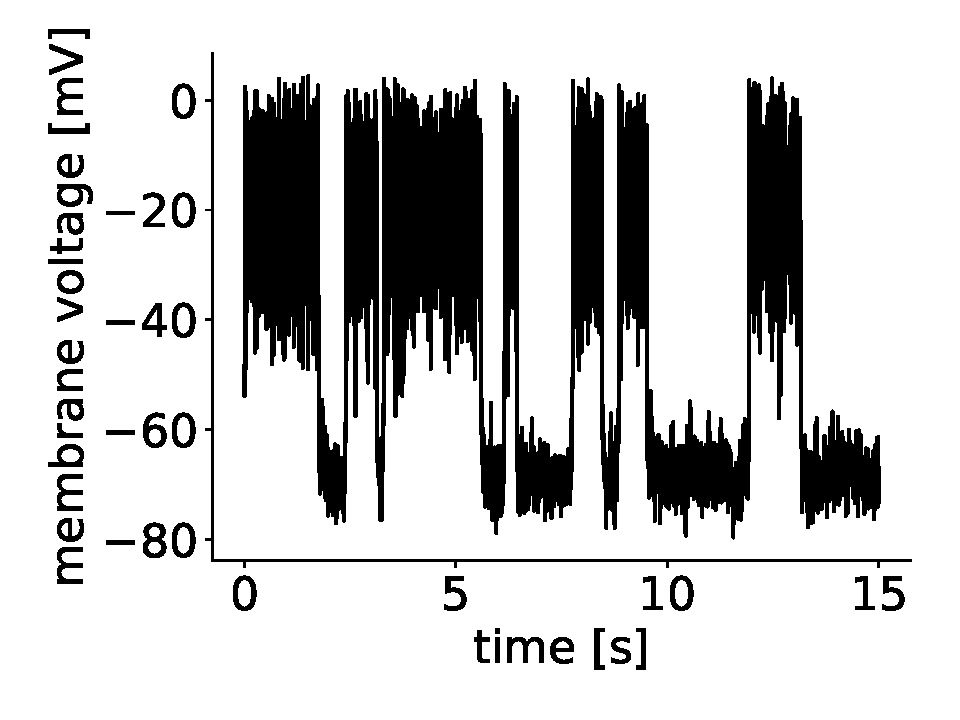
\includegraphics[scale=0.45]{realstatevar14vsh2noleg.pdf}}	\subfigure[]{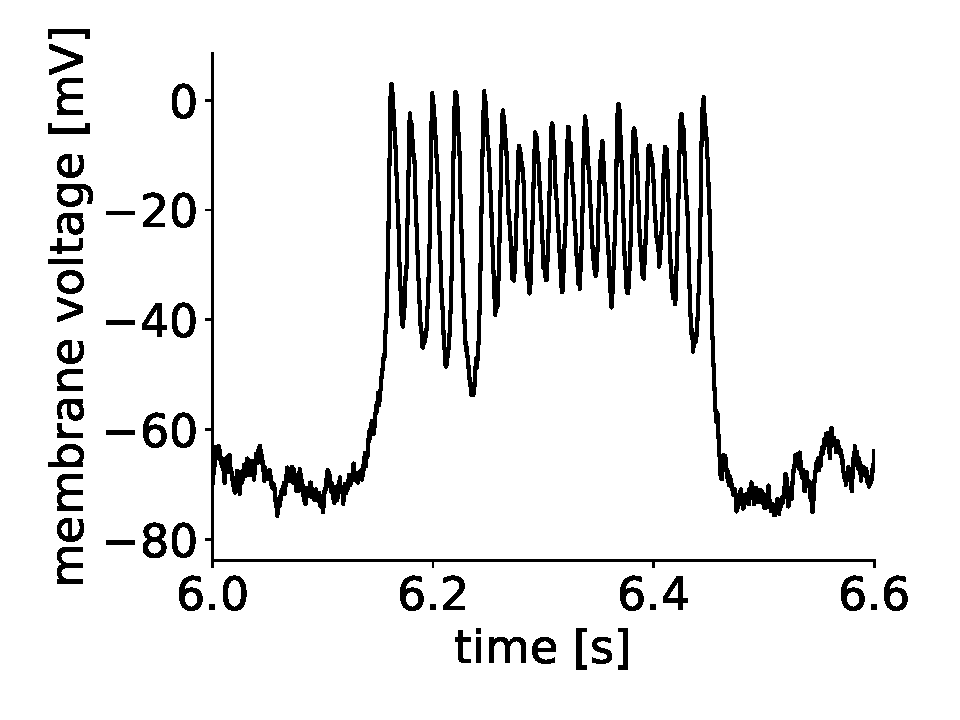
\includegraphics[scale=0.45]{realstatevar14v2noleg.pdf}} 
	\caption{Example of bistable membrane voltage under the influence of noise. The amplification in (b) illustrates the different qualitative behaviors in both regimes.}
	\label{bistablevolt} 
\end{figure}

A similar bistability has been observed for Brownian Particles in a tilted periodic potential, obeying the following equations of motion\cite{bpp}: 
\begin{equation}
\dot{v}=-\gamma v-U'(x)+\sqrt{2\gamma kT}\xi(t)
\end{equation}
with the potential $U(x)=-Fx-d\cos(x)$. $\gamma$ is the friction coefficient, $kT$ the thermal energy which corresponds to the noise intensity and the bias force $F$ determines the tilt of the potential.
\\
Assuming that friction is low and $F$ is chosen such that the tilted potential keeps its minima and maxima, the Brownian particle can be in two different velocity states (figure \ref{veldynintro}). If it performs noise-induced oscillations near a minimum, it is in the so-called \textit{locked state}. After the Brownian particle has managed to overcome a hill and still has enough energy to pass the adjacent maxima as well, it is said to be in the \textit{running state}. While making its way down the washboard potential, the Brownian particle constantly switches between these states due to the influence of noise.

\begin{figure}[H]
	\subfigure[]{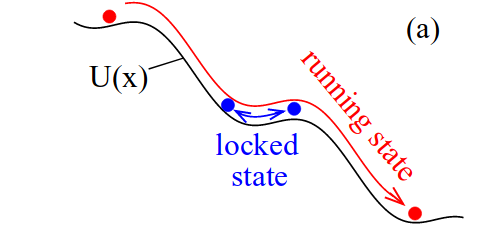
\includegraphics[width=0.5\textwidth]{veldynupper.png}} 
	\subfigure[]{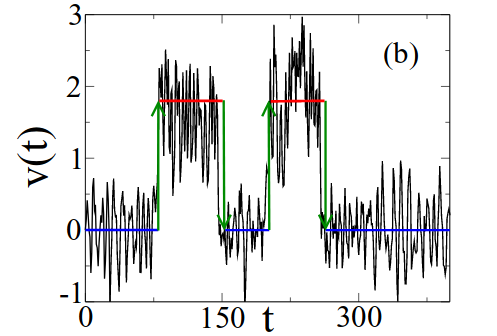
\includegraphics[width=0.5\textwidth]{veldynlower.png}} 
	\caption{Figure (a) visualizes the two motional states of a Brownian Particle in a periodic potential, on the right one can see the bistable velocity dynamics. The oscillations in the locked state are noise-induced while they mainly arise from local extrema of the potential in the running state. These images have been taken from\cite{bpp}.}
	\label{veldynintro} 
\end{figure}

In the case of large friction or a strongly tilted potential, however, the particle will barely move or move almost all of the time, respectively. In either configuration, one of the states prevails. When a couple of Brownian Particles are thrown into the system under these conditions, the majority of particles finds itself in the same state of motion. As a consequence, the particles move roughly as a group with only little spread around the mean velocity. Therefore, the effective diffusion coefficient $D_{eff}$ which quantifies the diffusional spread,
\begin{equation}
D_{eff}=\lim_{t\rightarrow\infty}\frac{\left\langle x^2(t) \right\rangle-\left\langle x(t)\right\rangle ^2}{2t}
\end{equation}
becomes very small. The other extreme case is reached when the parameters are chosen in such a way that both states are equally likely. Then, approximately half of the particles are resting while the others are in the running state, leading to a large $D_{eff}$. The lower the noise intensity, the fewer switchings occur and the higher is the effective diffusion coefficient. This phenomenon can be seen in figure (\ref{anbpsimintro}).

\begin{figure}[H]
	\centering
	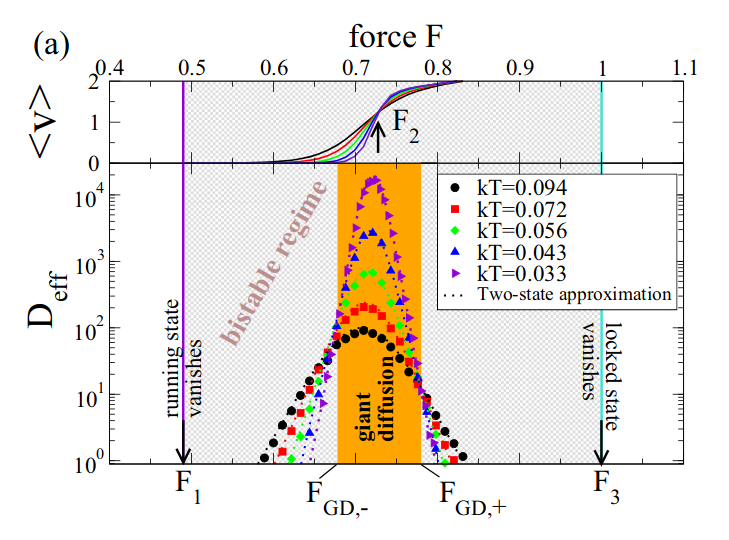
\includegraphics[scale=0.5]{nbpsim1.png}\caption{Simulation of velocity and effective diffusion coefficient for Brownian Particles in a tilted periodic potential,taken from \cite{bpp}}
	\label{anbpsimintro}
\end{figure}

The upper part of the picture shows the average velocity which naturally increases with the slope of the potential. Depending on the friction, there is a bias force - here denoted by $F_2$ - where frictional loss and acceleration via the potential annihilate each other. In the zero-noise limit, bias forces which are smaller than this value lead to a vanishing velocity, as the running state cannot be sustained without noise. The same argument can be made for $F>F_2$: as the running state cannot be stopped without noise, the maximum velocity is achieved. Consequently, all velocity curves make a jump and intersect each other at $F_2$.\\
As explained above, the diffusion coefficient gets maximal when both states are occupied with equal probabilities, which obviously happens at $F_2$. Interestingly, the Giant Diffusion is not only restricted to this particular bias force, but extends over a finite area between the two intersection points of all curves, $F_{GD,\pm}$. Outside of this region, $D_{eff}$ decreases with the noise intensity. It should be noted that a motion with low diffusion as it occurs outside the region of Giant Diffusion does not require the disappearance of one of the states, but happens much earlier. Thus, not all particles need to be in the same motional state to accomplish a small diffusion.
In order to better understand what happens in the bistable regime, a simplified description can be used. 
In the case of low noise intensity, the transition times between the locked state and the running state will be much shorter than the periods of time that the particle stays in one of the two states. That is why it is practical to describe the behavior of the system with a two-state model. The results of this model are plotted as dotted curves and show good agreement with the data. The transition rates between the states are assumed to obey an Arrhenius law:
\begin{align}\label{arrhlaw}
r_{\pm}=r_{0,\pm}\exp\left(-\frac{\Delta U_{\pm}}{D}\right)
\end{align}
where $r_-$ denotes the transition rate from locked to running state, and $r_+$ the rate for the other transition. $\Delta U_{\pm}$ is the corresponding potential barrier that needs to be traversed and $D$ the noise intensity which previously was $kT$. The effective diffusion coefficient can be calculated from the velocity $v_0$ in the running state and the transition rates\cite{abp}: 
\begin{align*}
D_{\text{eff}}=\frac{v_0^2 r_+r_-}{(r_++r_-)^3}
\end{align*}
This formula allows us to find the intersection points of the diffusion coefficients. As the curves for all noise intensities go through these points, they become independent of the noise intensity there.
It is
\begin{align*}
D_{\text{eff}}&=\frac{v_0^2r_{0,+}r_{0,-}\exp\left(-\frac{\Delta U_++\Delta U_-}{D}\right)}{\left[r_{0,+}\exp(\frac{-\Delta U_+}{D})+r_{0,-}\exp\left(\frac{-\Delta U_-}{D}\right)\right]^3}\\&=\frac{v_0^2r_{0,+}r_{0,-}}{\left[r_{0,+}\exp\left(-\frac{3\Delta U_+-\Delta U_+-\Delta U_-}{3D}\right)+r_{0,-}\exp\left(-\frac{3\Delta U_--\Delta U_+ -\Delta U_-}{3D}\right)\right]^3}\\&=\frac{v_0^2r_{0,+}r_{0,-}}{\left[r_{0,+}\exp\left(-\frac{2\Delta U_+-\Delta U_-}{3D}\right)+r_{0,-}\exp\left(-\frac{2\Delta U_--\Delta U_+}{3D}\right)\right]^3}
\end{align*}
In the limes $D\rightarrow 0,\Delta U_+>U_-$ the first term in the denominator vanishes, resulting in:
\begin{align*}
D_{\text{eff}}=\frac{v_0^2r_{0,+}}{r_{0,-}^2}\exp\left(-\frac{\Delta U_+-2\Delta U_-}{D}\right)
\end{align*}
Under the assumption that the prefactors change slowly in comparison to the exponential function, the following condition arises:
\begin{align}\label{fcrit}
\Delta U_+=2\Delta U_-
\end{align}
Due to symmetry of the problem, the opposing case $D\rightarrow 0,\Delta U_+<U_-$ yields:
\begin{align*}
\Delta U_-=2\Delta U_+
\end{align*}
In both cases, one potential barrier is twice as high as the other one.\\
The verification of this criterion requires knowledge of potential barriers. As there are no actual potential barriers in the system, it is only possible to derive effective barriers from the behavior of the system.
These can be acquired by measuring transition rates at different noise intensities and fitting them with the Arrhenius law from (\ref{arrhlaw}), as it was done in Figure \ref{ratesintro}.
\begin{figure}[H]
	\subfigure[]{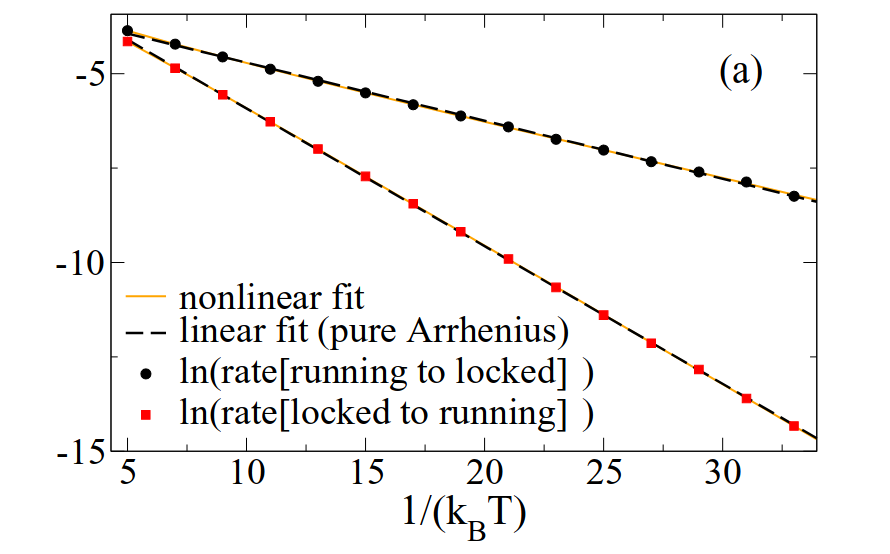
\includegraphics[width=0.5\textwidth]{kramerfit.png}} 
	\subfigure[]{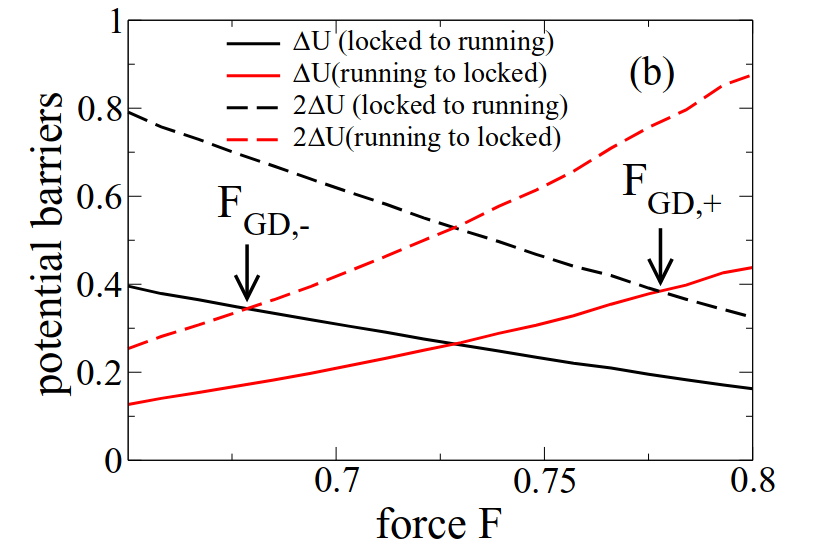
\includegraphics[width=0.5\textwidth]{barrierplot.png}} 
	\caption{The left shows the transition rates for a fixed bias force over a range of different noise intensities. Fits were done with both an Arrhenius and a Kramers law but yielded similar results for the effective barriers. On the right one can see the effective potential barriers, where the dotted curves are simply twice the solid curves.  The images have been taken from \cite{bpp}.}
	\label{ratesintro} 
\end{figure}
It can be seen that the Arrhenius-like behavior continues over a wide range of noise intensities, allowing to get reliable values for the effective potential barriers. According to the criterion from (\ref{fcrit}), the critical forces are expected to be at 0.68 and 0.76, which roughly corresponds to the actual intersection points.\\
Consequently, the bistable system at hand could be well described by the two-state theory. This implies that other resembling systems might show similar behavior, as for example bistable neurons. The quantities corresponding to position and velocity would be spike count and firing rate, and the noise source wouldn't be the temperature anymore, but channel noise or random input from surrounding neurons.
Instead of a critical bias force, there would be a critical bias current which needed to be crossed to reach Giant Diffusion. One of the most important aspects of this similarity would be signal transmission. If the system is driven by a slow cosine signal with amplitude $\epsilon$, the signal-to-noise ratio can be computed via
\begin{align*}
SNR=\frac{\epsilon ^2T}{8}\frac{|\chi(0)|^2}{D_{eff}}
\end{align*}
where $T$ denotes th total simulation time. Near the critical current, the spike count diffusion would change by multiple orders of magnitude, leading to a similar change in the SNR. \\
All in all, bistable neuron models are suggested to exhibit Giant Diffusion and therefore possess critical currents. When the system is near such a critical point, slight changes in the bias current can cause great changes in the SNR and possibly a large enhancement of signal transmission. The goal of this thesis is to find out whether Giant Diffusion exists for neuron models, to identify the critical currents and to investigate the system under the influence of slow periodic signals. 

\section{Models and Methods}
\subsection{The $I_{Na,p}+I_K$ model with saddle-node bifurcation}
The main focus of this thesis lies on the study of the $I_{Na,p}+I_K$-model, the persistent sodium plus potassium model with additive noise:
\begin{align}\label{Veq}
C\dot{V} &= I - g_L(V-E_L) - g_{Na}m_{\infty}(V)(V-E_{Na}) - g_Kn(V-E_K)+\sqrt{2D}\xi(t)\\\label{neq}
\dot{n} &= (n_{\infty}(V)-n)/\tau(V)
\end{align}
Here, $V$ denotes the membrane voltage, $C$ is the capacitance, $I$ is the bias current, $g_i$ are conductances and $E_i$ the Nernst equilibrium potentials. The overall noise intensity is $D$. Lastly, $m_{\infty}$ is the activation variable of the instantaneous $Na^+$ current, while $n$ governs the variation of the slower $K^+$ current. The steady-state activation functions are approximated by the Boltzmann-function:
\begin{align*}
f_{\infty}(V) = \frac{1}{1+\exp\{(V_{1/2}-V)/k\}}
\end{align*}
At $V_{1/2}$, the activation function has the value 1/2, and $k$ is the slope factor determining the steepness around $V_{1/2}$ - a smaller value of $k$ leads to a more abrupt change of $f_{\infty}$. This approximation was suggested by Izhikevich \cite{izi}.\\
The fastest neural oscillations in the human brain are gamma waves with frequencies in the range between 25 and 100 Hz\cite{gamma}\cite{gamma2}. Similar values can also be found in different papers about bursting neurons\cite{burstneu}\cite{burstneu2}. Therefore, the parameters were chosen such that the frequency in the bursting state was about 70 Hz.
The exact values used in the simulations were:\\\\
$C=1$ , $g_L=0.3$ , $E_L=-80$ , $g_{Na}=1$ , $E_{Na}=60$ , $g_K=0.4$ , $E_K=-90$.
\begin{align*}
\intertext{Instantaneous $Na^+$ current:} k_m&=14 , V_{1/2,m}=-18. 
\\
\intertext{$K^+$ current:} k_n&=5 , V_{1/2,n}=-25 , \tau(V)=\text{const}=3.
\end{align*}
%\subsubsection{Phase plane analysis}
\subsubsection{System without noise}\label{mod1won}
The qualitative behavior of the neural model can be best understood by first considering the noiseless system.
For a system that depends on the evolution of two state variables, in this case $V$ and $n$, some qualitative and quantitative analysis can be carried out in the phase plane. A neat way to obtain information about an unknown system is to calculate its nullclines. The nullclines are curves in the phase plane, where one of the state variables remains constant. Thus, the $V$-nullcline is defined by the condition $\dot{V}=0$ and the $n$-nullcline follows from $\dot{n}=0$. By crossing one of the nullclines, the system changes its direction of motion with respect to the corresponding variable. As a consequence, each nullcline separates the phase space into two regions where one of the variables evolves in opposite directions. Taken together, the nullclines define four different regions of directions: one region each where both variables decrease or increase and two regions where one variable increases and the other decreases. Depending on the specific shape of the nullclines, these regions do not necessarily have to be coherent.\\
The $V$-nullcline can be obtained by setting the left side of equation (\ref{Veq}) to zero. In the $V$-$n$-plane, it can then be described by the function
\begin{align}
n(V)=\frac{I - g_L(V-E_L) - g_{Na}m_{\infty}(V)(V-E_{Na})}{g_K(V-E_K)}
\end{align} 
The $n$-nullcline is just
\begin{align}
n(V)=n_\infty(V)
\end{align}
The nullclines of the $I_{Na,p}+I_K$-model are shown in figure \ref{realnc}.\\
A second aspect of the nullclines are their intersection points. As both state variables remain constant when the nullclines intersect, these points are equilibrium points.\\
In general, there are three different types of equilibria: nodes, saddles and foci. These may be stable or unstable. Any trajectory in the phase space starting close enough to a stable equilibrium stays near it for all times. In contrast to that, an equilibrium is unstable, if at least one trajectory that starts arbitrarily close to it diverges from the equilibrium.
If they are in the vicinity of a node, all trajectories either converge to or diverge from it. In the case of a saddle, most trajectories first approach the equilibrium point and then diverge from it. Trajectories that start near a focus rotate around the equilibrium point and thereby get closer to or farther away from it. 
%\subsubsection{Jacobian matrix of the system}
The equilibrium points can be characterized by studying the Jacobian matrix of the system at these points. A two-dimensional system can be written in the form
\begin{align}
\dot{x}=f(x,y)\\
\dot{y}=g(x,y)
\end{align}
Utilizing the fact that the functions $f$ and $g$ can be linearized near the equilibrium, which means they can be approximated by the first term of their Taylor expansion, one finds a linear system at the equilibrium $(x_0,y_0)$:
\begin{align}				
\left(\begin{matrix}\dot{u}\\\dot{w}
\end{matrix}\right)
=\left(\begin{matrix}a\quad b\\
c\quad d\end{matrix}\right)\left(\begin{matrix}u\\w\end{matrix}\right)=L\left(\begin{matrix}u\\w\end{matrix}\right)
\end{align}
where $u=x-x_0$, $w=y-y_0$, $L$ is the Jacobian matrix at equilibrium and the coefficients are the partial derivatives
\begin{align}
a=\frac{\partial f}{\partial x}(x_0,y_0),\qquad b=\frac{\partial f}{\partial y}(x_0,y_0) \\
c=\frac{\partial g}{\partial x}(x_0,y_0),\qquad d=\frac{\partial g}{\partial y}(x_0,y_0)
\end{align} 
Having determined the eigenvalues $\lambda_\pm$ and eigenvectors $ \boldsymbol{v_\pm}$ of $L$, a solution for the linear system can be constructed:
\begin{align}
\left(\begin{matrix}u(t)\\w(t)
\end{matrix}\right)=c_+\boldsymbol{v_+}\exp(\lambda_+t)+c_-\boldsymbol{v_-}\exp(\lambda_-t)
\end{align}
At this point, the connection between the Jacobian matrix and the different types of equilibria becomes clear. If both eigenvalues are real and have the same sign, both terms of the solution either grow or decay exponentially, meaning that the equilibrium is a node. If they are real with opposite signs, the equilibrium point is a saddle. Finally, if the eigenvalues are complex-conjugate, the solution oscillates, which makes the equilibrium a focus\cite{izi}.\\
When no bias current is applied (that is, I=0), the system features three equilibrium points:
\begin{figure}[H]
	\centering
	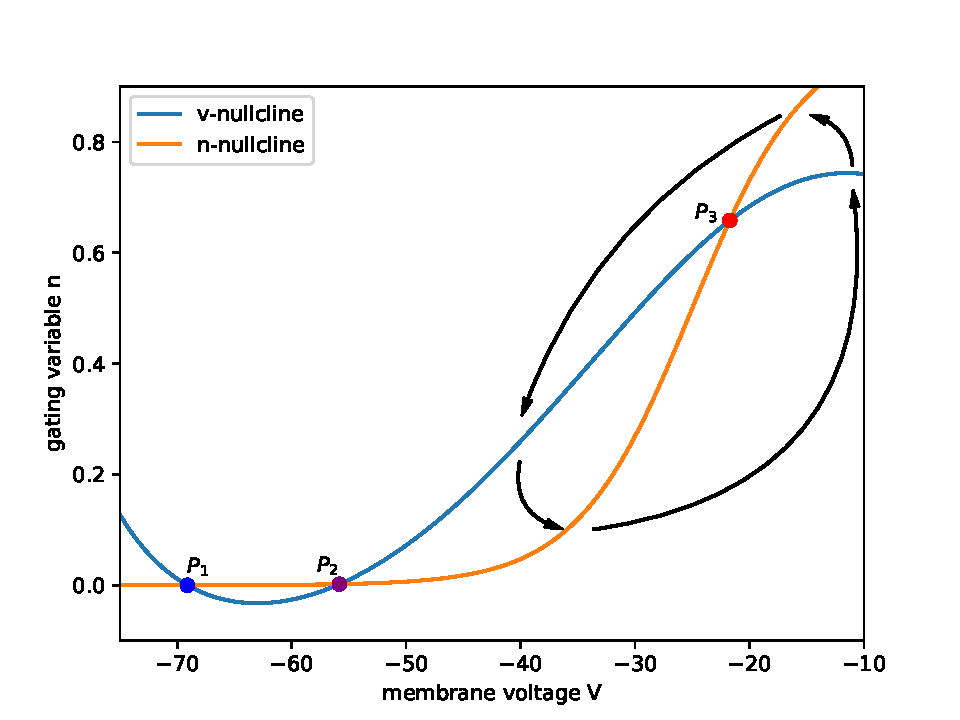
\includegraphics[scale=0.5]{inapikrealncwnp.pdf}\caption{Nullclines of the $I_{Na,p}+I_K$-model with $I=0$. The arrows indicate the direction of motion in the different regions.}
	\label{realnc}
\end{figure}
Carrying out the phase plane analysis, one finds:
\begin{align*}
\lambda_+(P_1)&\approx-0.1 & \lambda_-(P_1)&\approx-0.3\\
\lambda_+(P_2)&\approx 0.1& \lambda_-(P_2)&\approx -0.3\\
\lambda_+(P_3)&\approx 0.05 + 0.5i& \lambda_-(P_3)&\approx 0.05 - 0.5i
\end{align*}
This means that $P_1$ is a stable node, $P_2$ is a saddle point and $P_3$ is an unstable focus. Thus, in the bursting state, the phase vector will rotate around $P_3$, approach $P_2$ in $n$ - direction and then go away from $P_2$ in $V$ - direction in order to do another rotation around $P_3$.\\
However, this applies only to the case of small bias currents. When $I\approx 0.36$, the saddle and the node fall together and the system undergoes a saddle-node bifurcation off invariant circle. In this case, the resting state vanishes and the neuron is in a state of tonic spiking.
\\
Provided that we are in the bistable regime, a system with arbitrary initial conditions will either go to the resting or the running state and will not change its behavior anymore after a short period of equilibration, as can be seen in figure \ref{subfig}. 
\begin{figure}[H]
	\subfigure[]{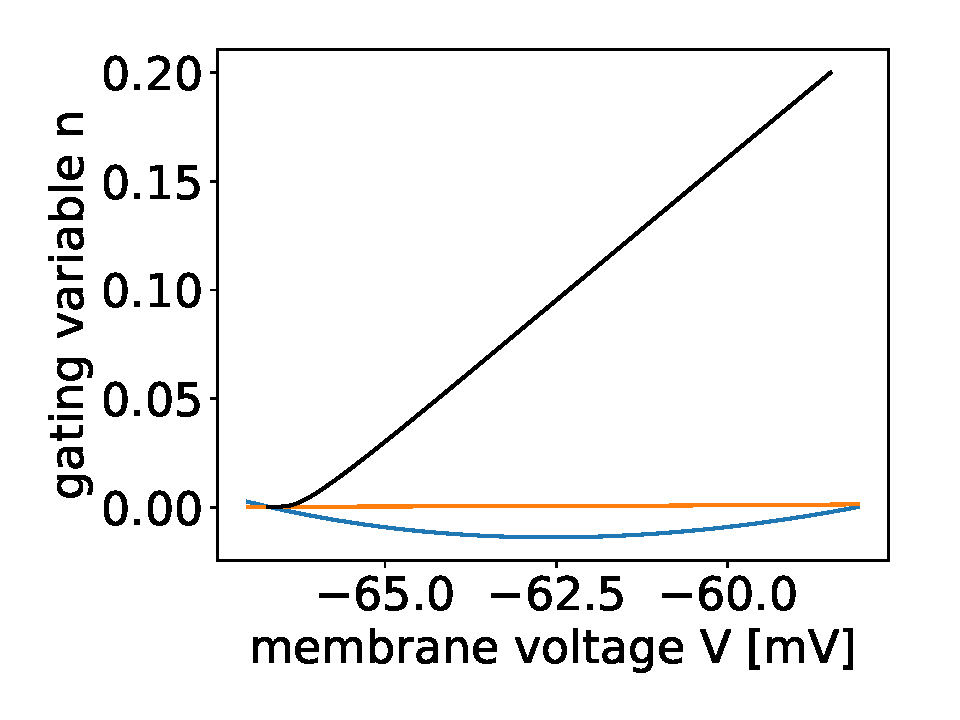
\includegraphics[scale=0.45]{inapreali20nbfontblack.pdf}} 
	\subfigure[]{	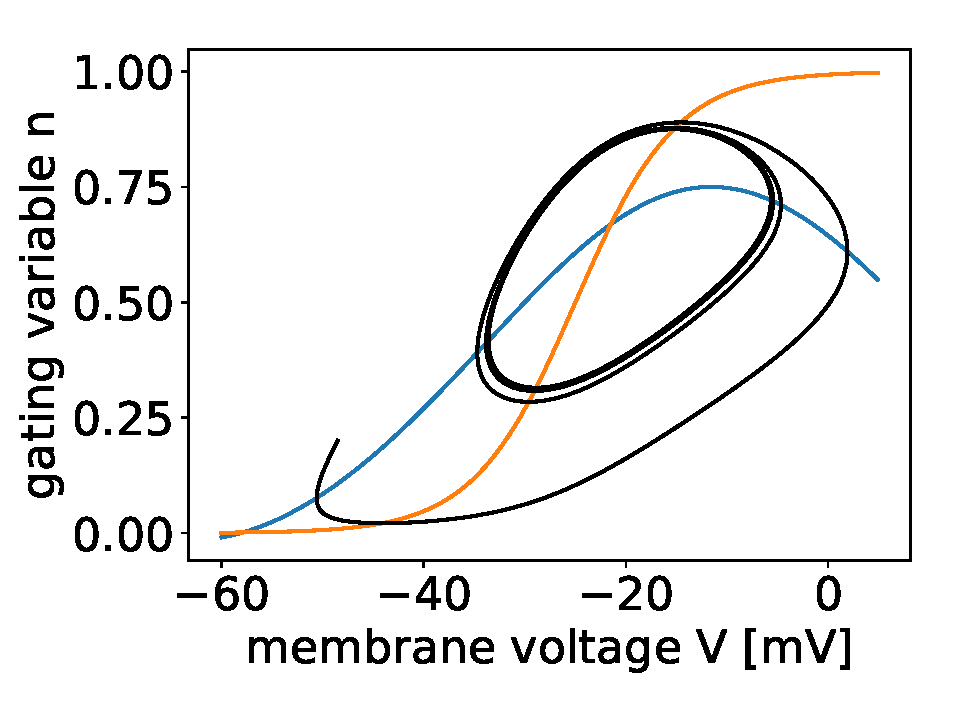
\includegraphics[scale=0.45]{inapreali20fontblack.pdf}}\\	\subfigure[]{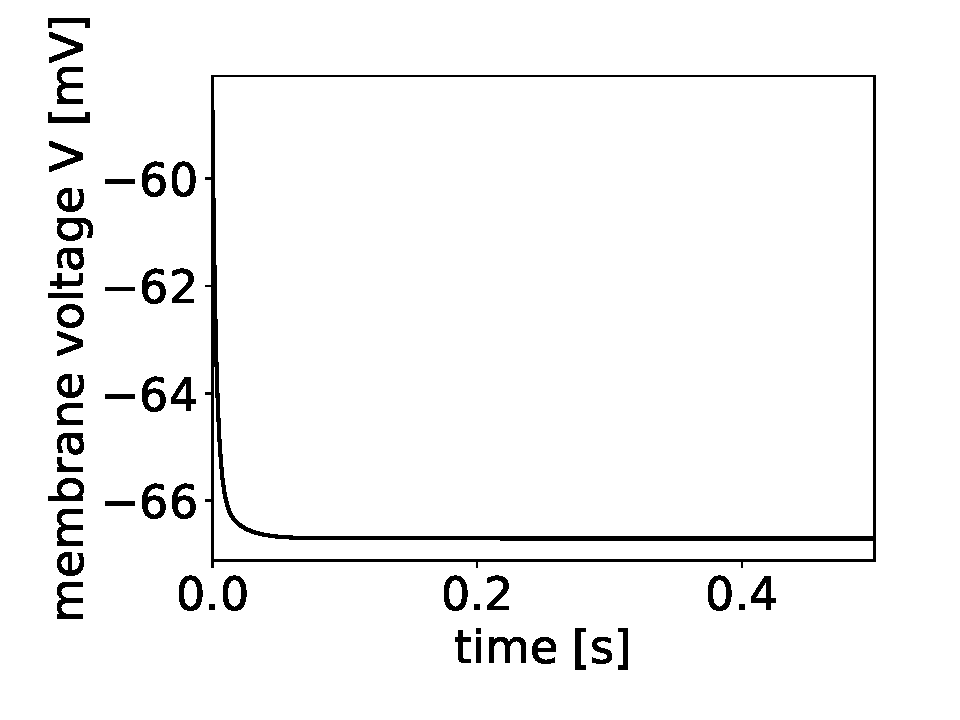
\includegraphics[scale=0.45]{inapreali20nbvfontblack.pdf}} 
	\subfigure[]{	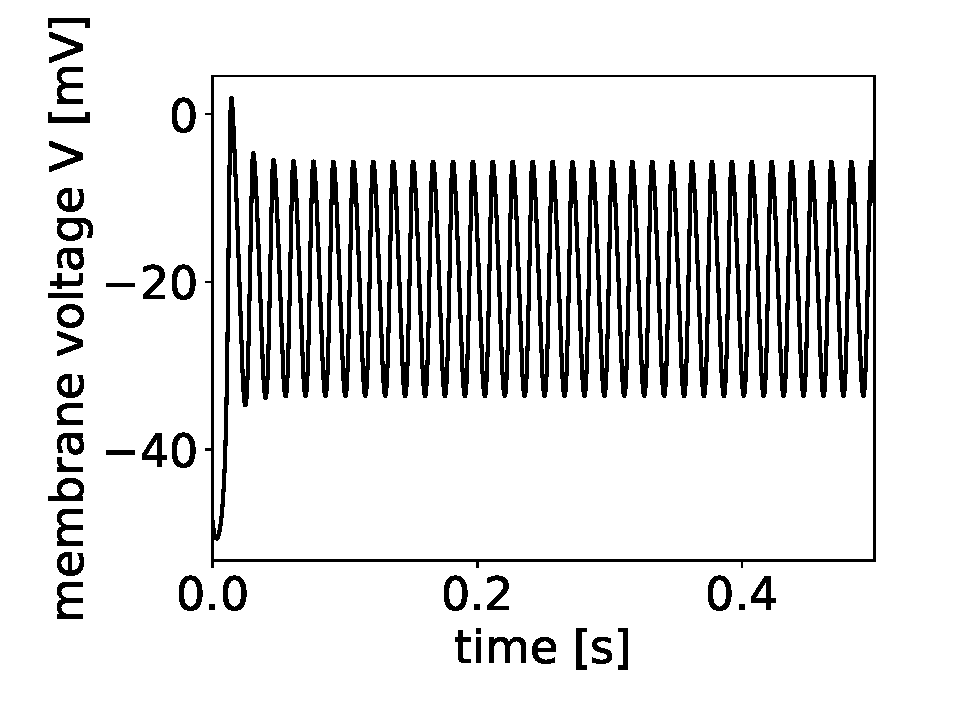
\includegraphics[scale=0.45]{inapreali20vfontblack.pdf}}
	\caption{Evolution of the phase vector (first row) and the membrane voltage over time (second row).
		The left side shows the evolution of the system with resting ICs, and on the right one can see the behavior under spiking ICs.}
	\label{subfig} 
\end{figure}
Analytically, it is hardly possible to determine whether a specific starting point ($V_0$,$n_0$) leads to repetitive spiking or no spiking at all. The only thing one can say for sure is that the line that separates both domains will go through the saddle point that was found in the phase plane analysis. Assuming that the gating variable does not change, any trajectory starting at higher voltages will lead to spiking while all trajectories at lower voltage converge to the stable node. A numerical investigation of the model without noise confirms our presumptions (figure \ref{twodom}).
\begin{figure}[H]
	\hspace*{-0.5cm}
	\subfigure[]{	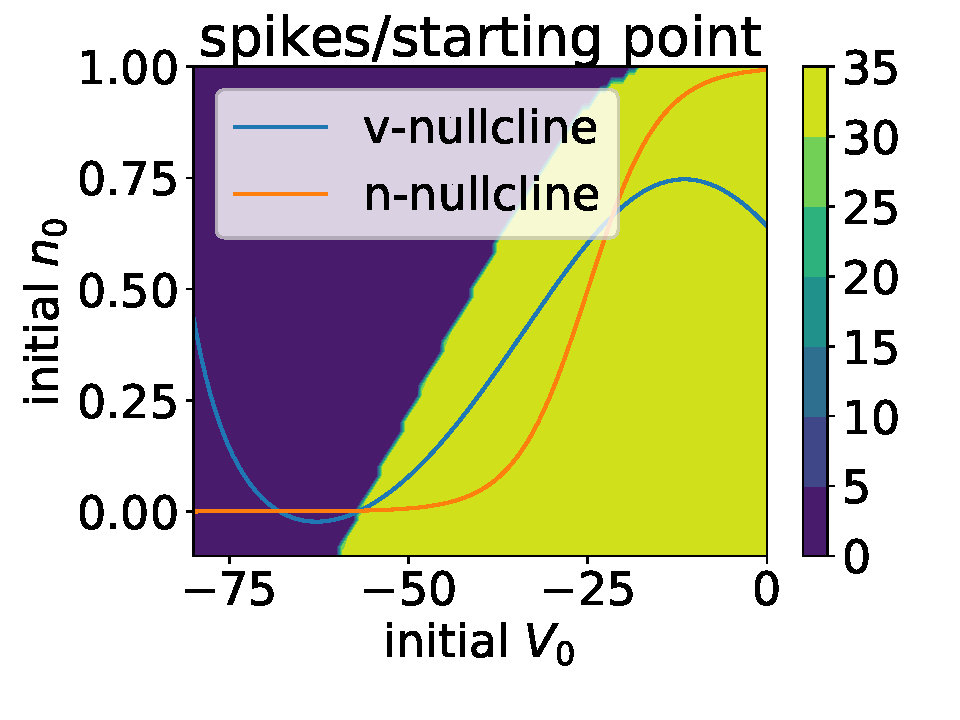
\includegraphics[scale=0.5]{contourtime01wn2.pdf}}
	\subfigure[]{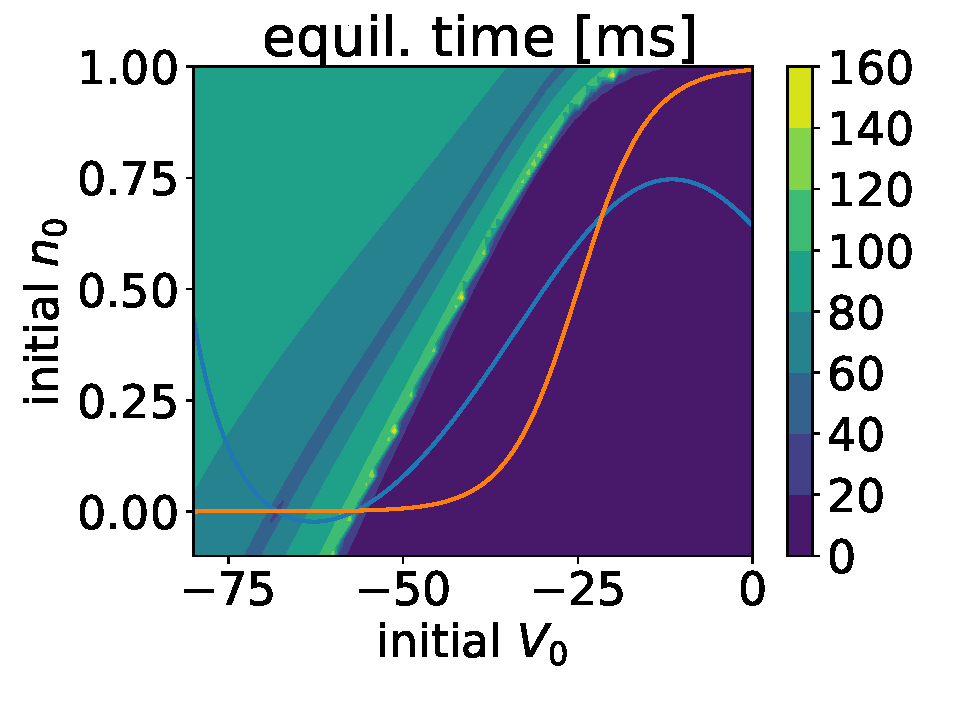
\includegraphics[scale=0.5]{contoureqtime01wn3.pdf}}
	
	\caption{Phase plane image of the neuron model with $I=0.1$ and no noise. Each point represents a specific combination of starting parameters. The left plot shows the number of spikes over a short period of time and for the right picture, the equilibration times for both states were measured. Irregularities arise from the finite resolution of the $V_0$-$n_0$-lattice.}
	\label{twodom}
\end{figure}		
There are two distinct regions which can be separated by a monotonically increasing curve that passes through the saddle point. In figure \ref{twodom}b one can see a small intermediate area of large equilibration times. If the system parameters lie in the vicinity of this transition area, a small perturbation suffices to bring the system into either state. Remarkably, most of this area is made up by starting points leading to the stable equilibrium while only a small streak consists of bursting initial conditions. Consequently, the running state is reached much faster than the resting state.
\subsubsection{System with noise}
When noise is brought into the system, the findings for the noiseless system still apply to a great extent. Starting in one of the two domains, the system will most likely first converge to the corresponding state, and the time it takes for that will be about the same as before. However, the system will not stay in this state forever, but constantly perform noise-driven transitions between the states. Thus, it will not be possible anymore to assign an end state to each set of initial conditions. Obviously, both transition rates, meaning from running to resting and in the opposite direction, will grow when the noise intensity $D$ increases. \\
In addition to that, depending on the overall configuration, the system is usually biased towards one of the states. It is to be expected that at low bias current $I$, the resting state dominates and the running state is favored at high $I$. Considering the simulations (figure \ref{currentnoise}), this turns out to be a valid hypothesis: At $I=-0.1$, the neuron almost immediately returns to the resting state once it has gotten into the running state. At a slightly higher bias current of $I=0$, the periods of stay in both states are almost equal, and at $I=0.15$, the system is in the running state for the majority of time. The firing frequency in the running state lies at about 70 Hz.
\begin{figure}[H]
	\subfigure[]{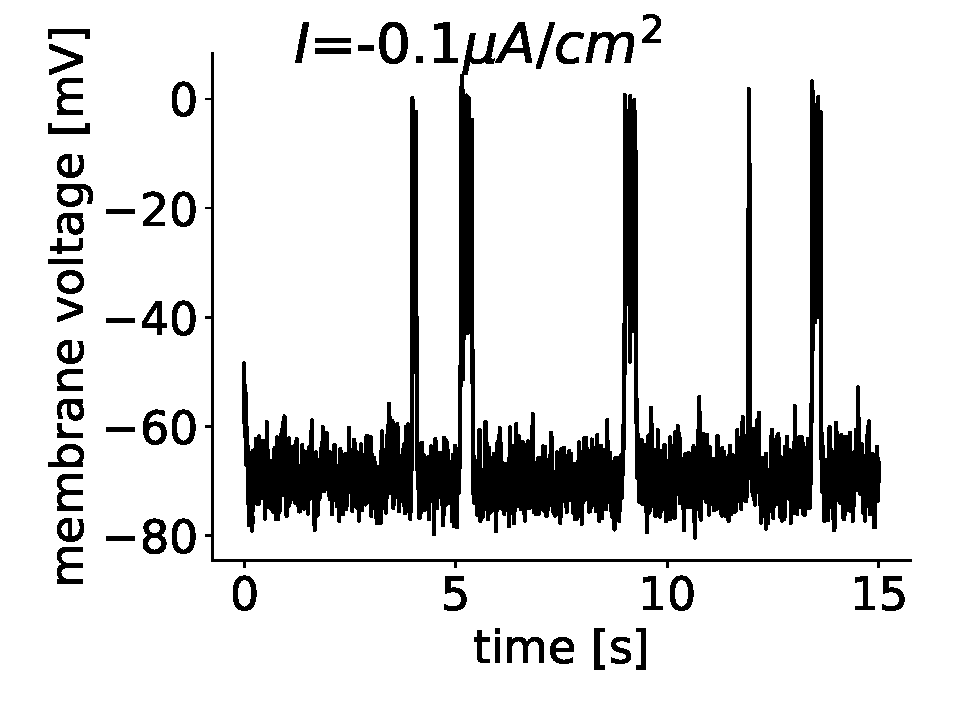
\includegraphics[scale=0.4]{realstatevar1252.pdf}} 
	\subfigure[]{	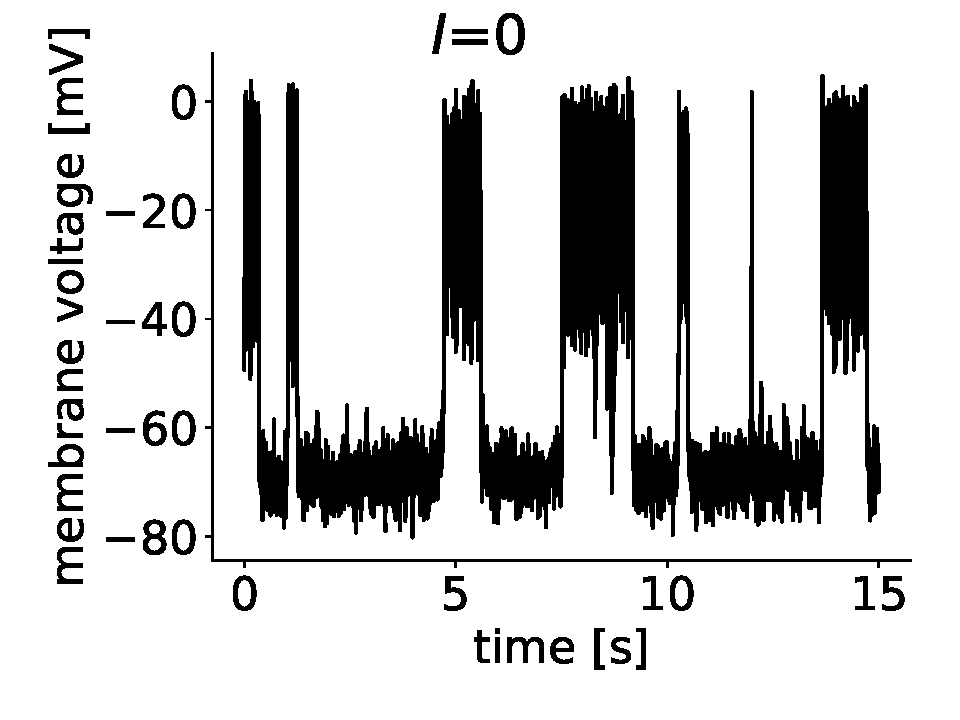
\includegraphics[scale=0.4]{realstatevar1352.pdf}}\\	\subfigure[]{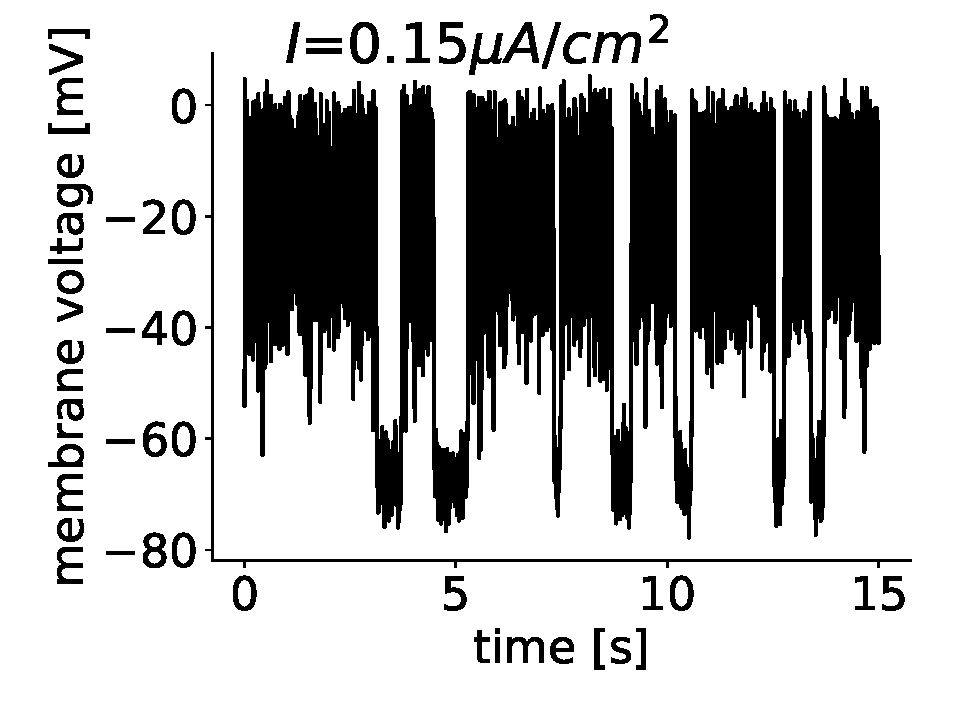
\includegraphics[scale=0.4]{realstatevar152.pdf}} 
	\subfigure[]{	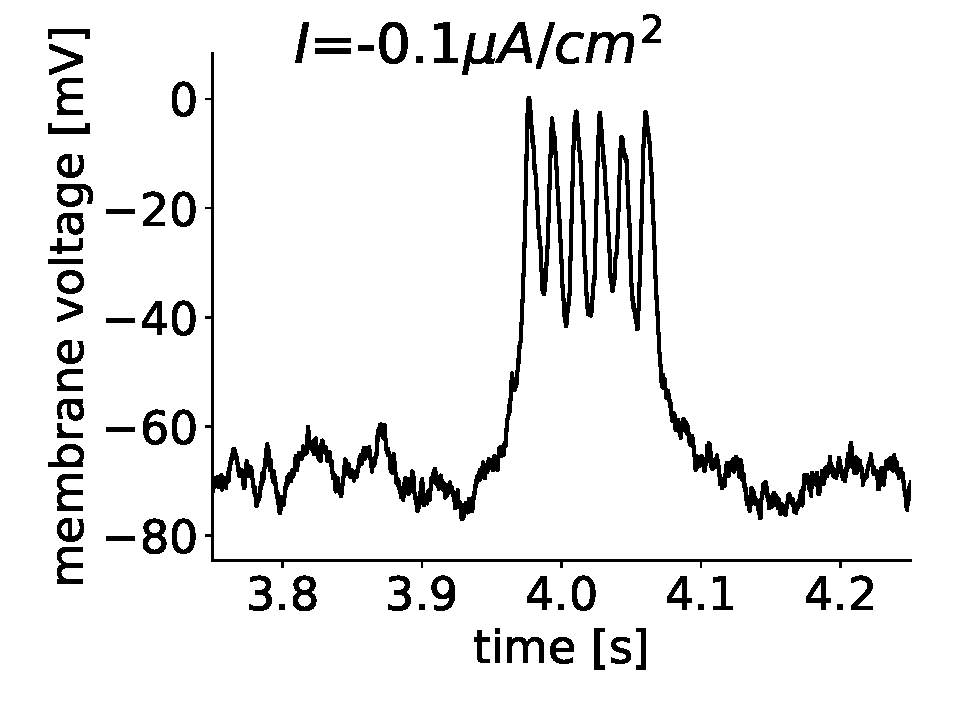
\includegraphics[scale=0.4]{realstatevar125vsh2.pdf}}
	\caption{Behavior of the membrane voltage for constant noise and changing bias current $I$. In figure (d), a segment with a higher time resolution is shown in order to better illustrate the evolution of the voltage variable.}
	\label{currentnoise} 
\end{figure}
In conclusion, the behavior of this two-dimensional bursting model displays the same characteristics as the Brownian particle in a tilted potential. Therefore, we expect to find similar count statistics and Giant Diffusion for this system as well. If this assumption is actually valid will be examined in the following chapter.
\subsubsection{System with periodic signal}
\subsection{$I_{Na,p}+I_K$ model with subcritical Andronov-Hopf bifurcation}
As we have now observed the phenomenon of giant diffusion and its implications in a two-dimensional neuron model, it is of particular interest to confirm this behavior also for other bistable two-dimensional neuron models. Finding out in which cases giant diffusion occurs may help to determine conditions that need to be fulfilled and eventually lead to experiments supporting these findings. Therefore two more models will be discussed in this section.
The first one is again the $I_{Na,p}+I_K$ model.
This model is very versatile and displays a wide variety of qualitative and quantitative behavior upon parametric adjustments. Thus, its features can be tweaked such that the system undergoes an Andronov-Hopf bifurcation when the bias current passes a certain value. As presented in section 3, the system is decribed by equations \ref{Veq} and \ref{neq}. The parameters now were the following:\\\\
$C=1$ , $g_L=1$ , $E_L=-78$ , $g_{Na}=4$ , $E_{Na}=60$ , $g_K=4$ , $E_K=-90$.
\begin{align*}
\intertext{Instantaneous $Na^+$ current:} k_m&=7 , V_{1/2,m}=-30. 
\\
\intertext{$K^+$ current:} k_n&=5 , V_{1/2,n}=-45 , \tau(V)=\text{const}=1.
\end{align*}
\subsubsection{System without noise}
Due to the parameter adjustments one obtains a slightly different phase space picture:
\begin{figure}[H]
	\centering
	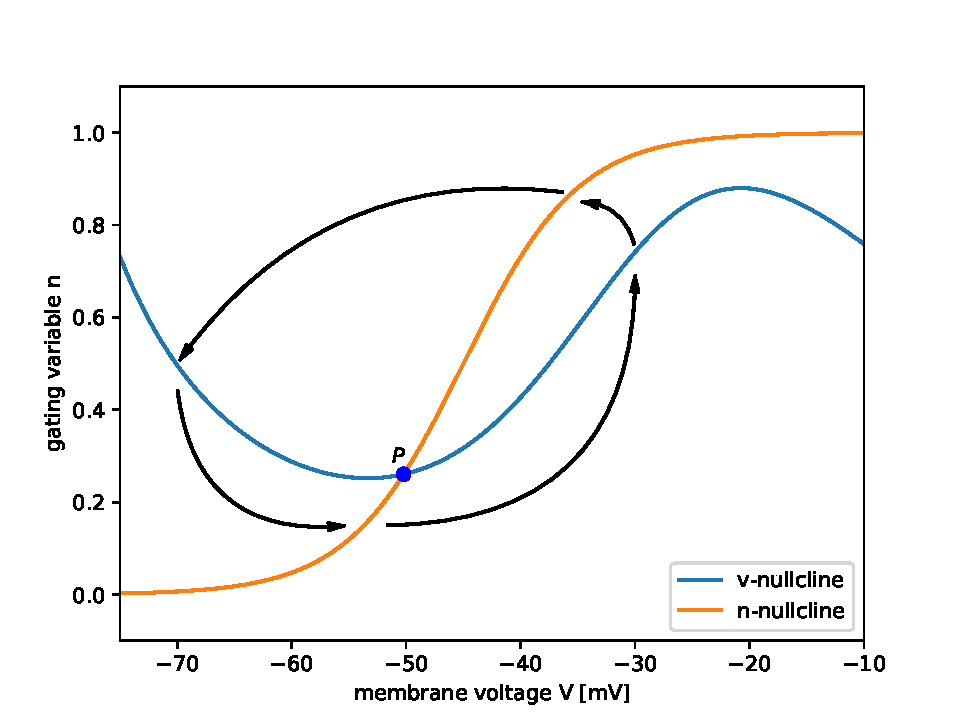
\includegraphics[scale=0.5]{inapikanhopfnc.pdf}\caption{Nullclines of the adjusted $I_{Na,p}+I_K$-model with $I=46$. The arrows indicate the direction of motion in the different regions.}
	\label{anhopfnc}
\end{figure}
The new nullclines yield only one equilibrum point. Computing the Jacobian matrix, following eigenvalues arise for this point:
\begin{align*}
\lambda_+(P)&\approx -0.05 + 2.3i& \lambda_-(P)&\approx -0.05 - 2.3i
\end{align*}
Complex eigenvalues with negative real parts indicate a stable focus. As before, the system performs large oscillations around the focus when it is in the running state. When it is near the equilibrium, it converges fast to it, with the exception that it doesn't approach it directly but oscillates around it with decreasing radius.
In contrast to the previous case, the system now not only consists of stable limit cycle and equilibrium but also an unstable limit cycle in between the two stable configurations. Considering that the system is under the influence of noise, it will not spend much time in the unstable state and quickly collapse into a stable configuration.\\
Upon increase of the bias current, the unstable limit cycle shrinks. At $I\approx 48.9$, it falls together with the stable equilibrium and makes it lose stability. This transition is called a subcritical Andronov-Hopf bifurcation.\\
While in the first model the states were characterized by oscillations around different equilibria, the state vector now only rotates around one equilibrium point. The current state can thereby be identified via the radius of the oscillations. Resting initial conditions result in a small radius and asymptotic convergence to the focus and spiking initial conditions just lead to regular firing with a larger radius, as can be seen in figure \ref{subfigah}.
\begin{figure}[H]
	\subfigure[]{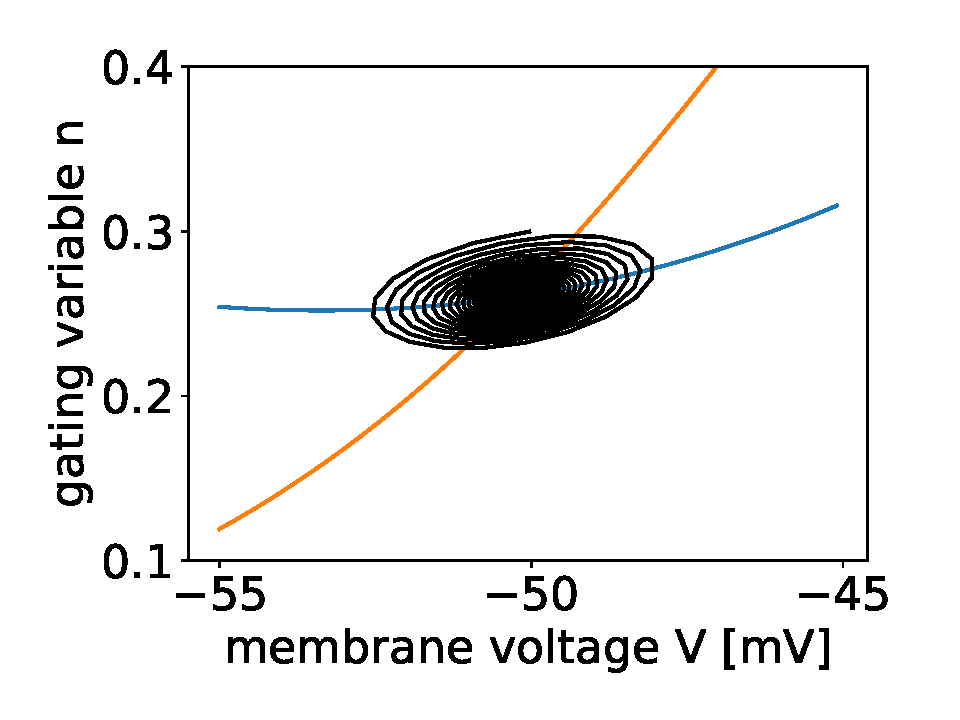
\includegraphics[scale=0.45]{inaprealanhopfnbblack.pdf}} 
	\subfigure[]{	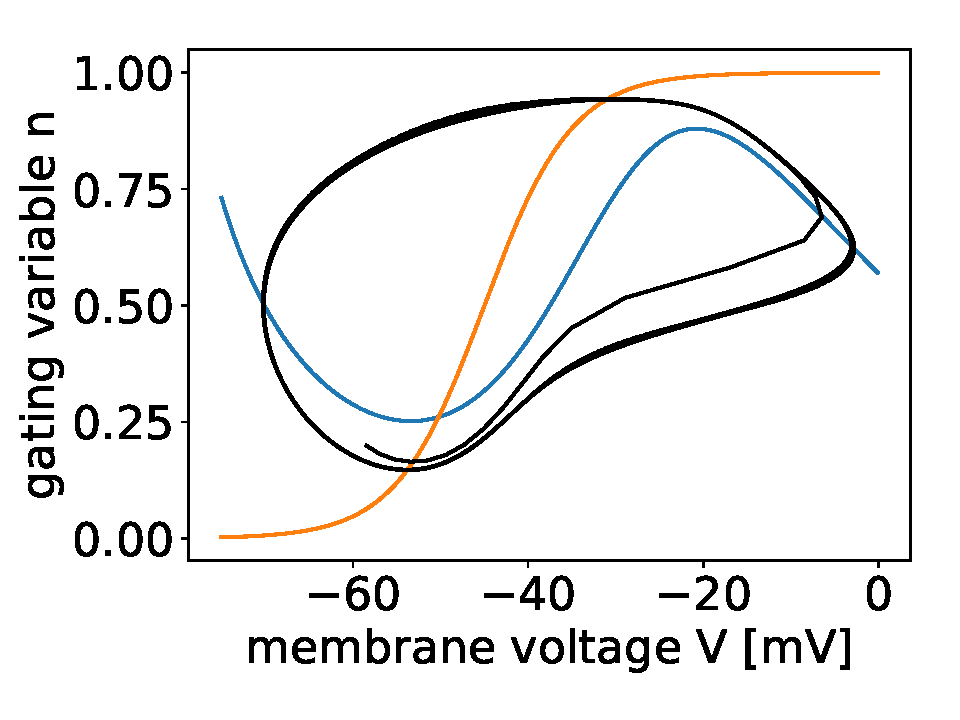
\includegraphics[scale=0.45]{inaprealanhopfblack.pdf}}\\	\subfigure[]{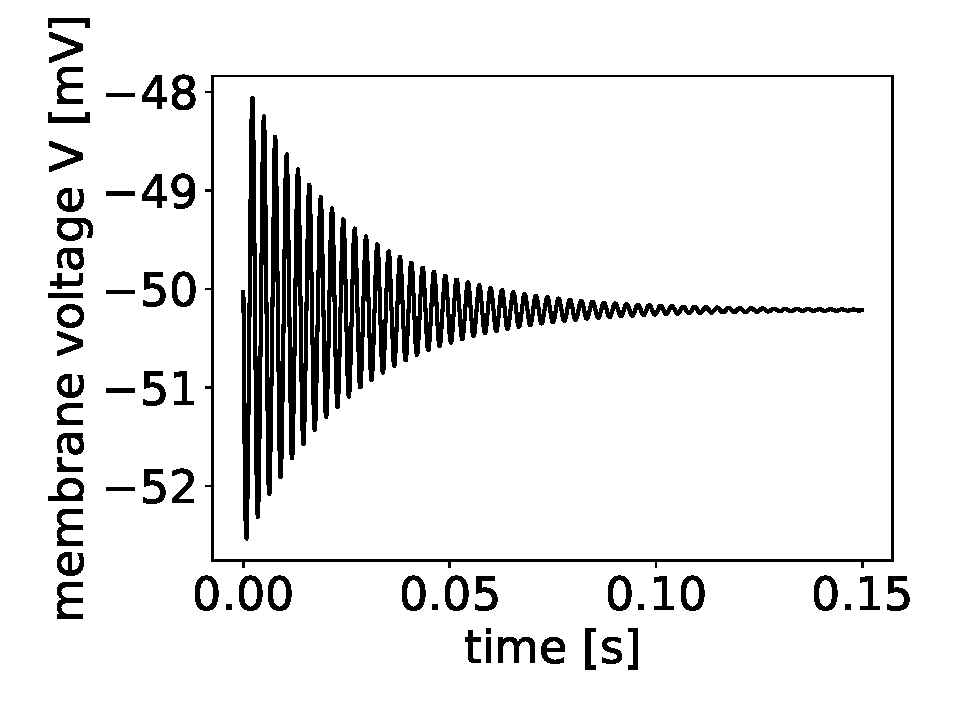
\includegraphics[scale=0.45]{inaprealanhopfnbvtblack.pdf}} 
	\subfigure[]{	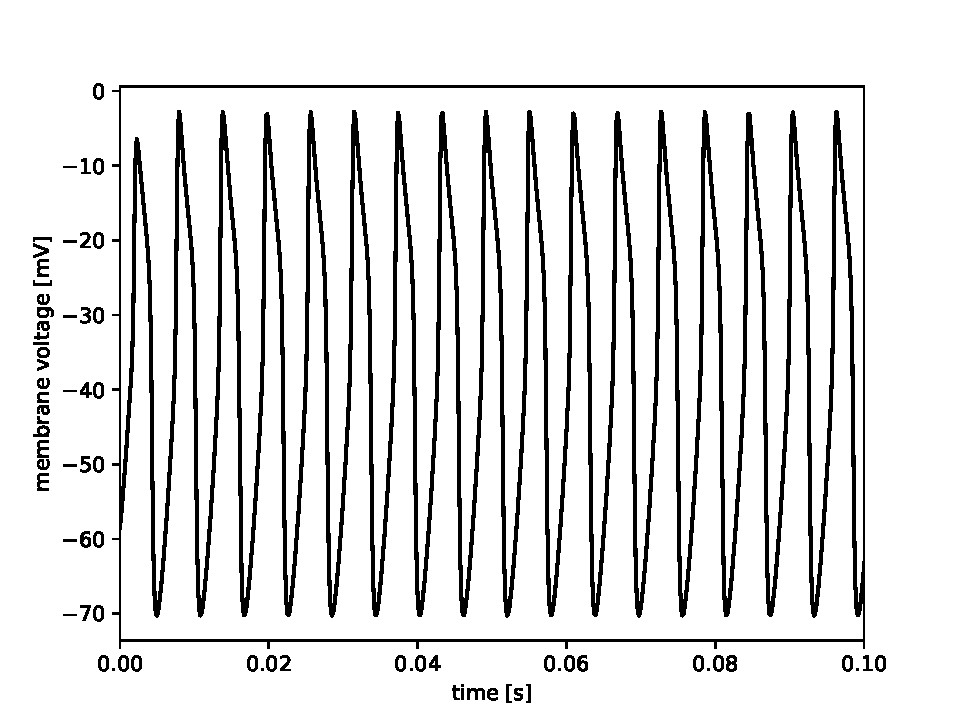
\includegraphics[scale=0.45]{inaprealanhopfvtblack.pdf}}
	\caption{Evolution of the phase vector (first row) and the membrane voltage over time (second row). The left side shows the evolution of the system with resting ICs, and on the right one can see the behavior under spiking ICs.}
	\label{subfigah} 
\end{figure}
In order to be able to distinguish between spiking and resting initial conditions, one may simulate the system at different starting points and see how it evolves, as has been done in section \ref{mod1won}.
\begin{figure}[H]
	\hspace*{-0.5cm}
	\subfigure[]{	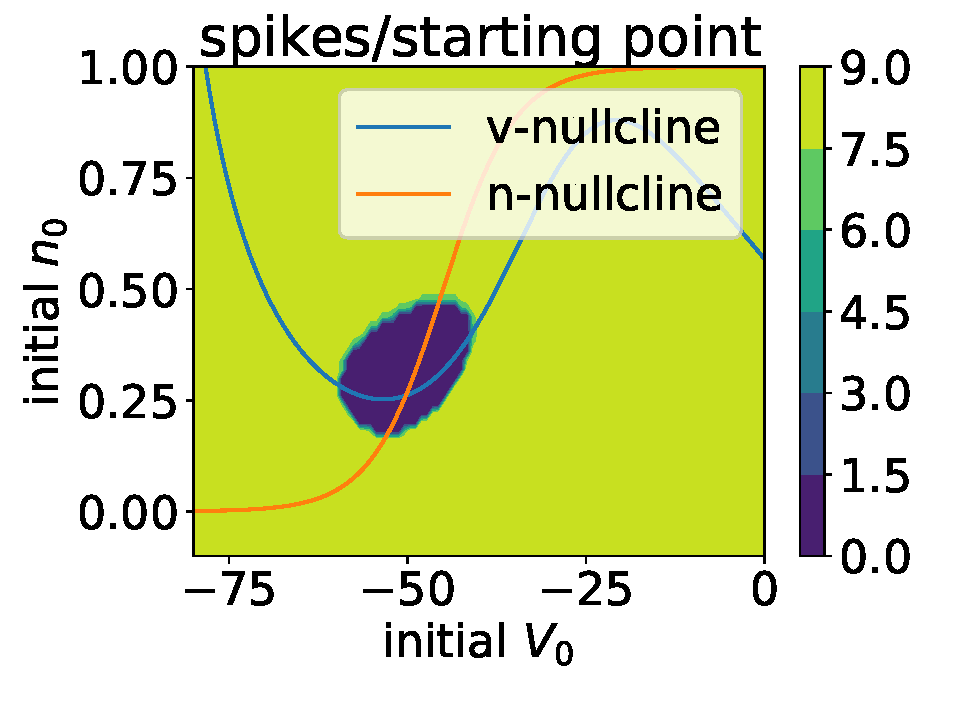
\includegraphics[scale=0.5]{contouranhopfa2sh.pdf}}
	\subfigure[]{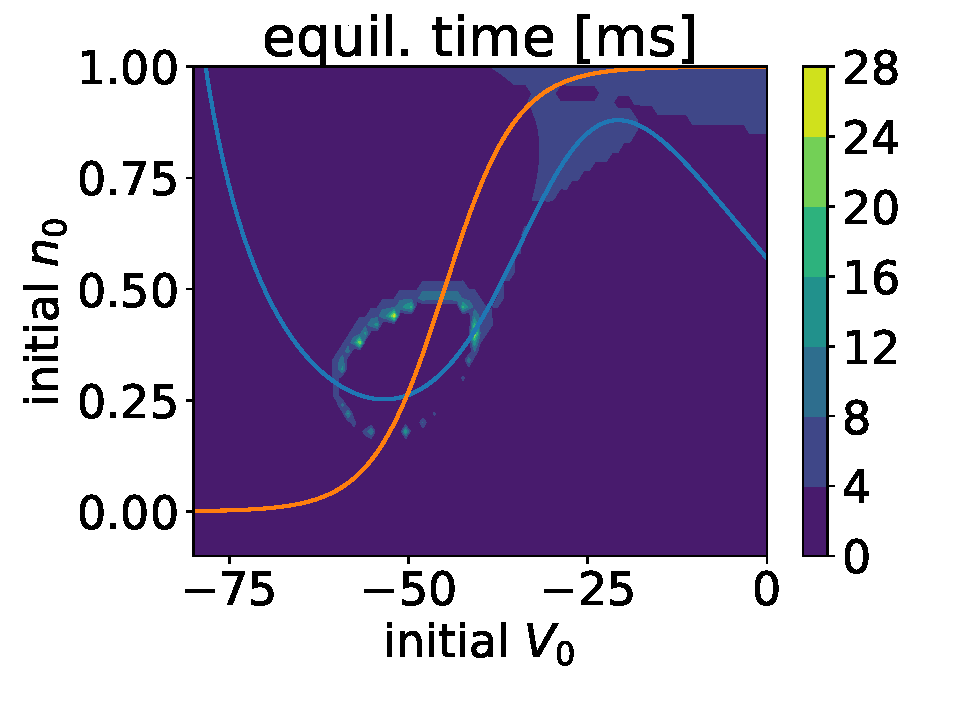
\includegraphics[scale=0.5]{contouranhopfa2time.pdf}}
	
	\caption{Phase plane image of the neuron model with $I=46$ and no noise. Each point represents a specific combination of starting parameters. The left plot shows the number of spikes over a short period of time and for the right picture, the equilibration times for both states were measured. In both images one can see the shape of the unstable limit cycle that separates both domains. Irregularities arise from the finite resolution of the $V_0$-$n_0$-lattice.}
	\label{twodom2}
\end{figure}
The area of resting initial conditions is completely enclosed by the spiking regime. Near the border, the system takes longer to equilibrate. This is due to the unstable limit cycle which separates both regimes. By crossing this ellipse from within or from the outside, the system goes over into the firing or resting state, respectively. The course of the unstable limit cycle can be seen in figure \ref{unstable}. These images were obtained by simulating the neuron model with negative time steps. That way, unstable regions are turned into stable ones and vice versa. 
\begin{figure}[H]
	\subfigure[]{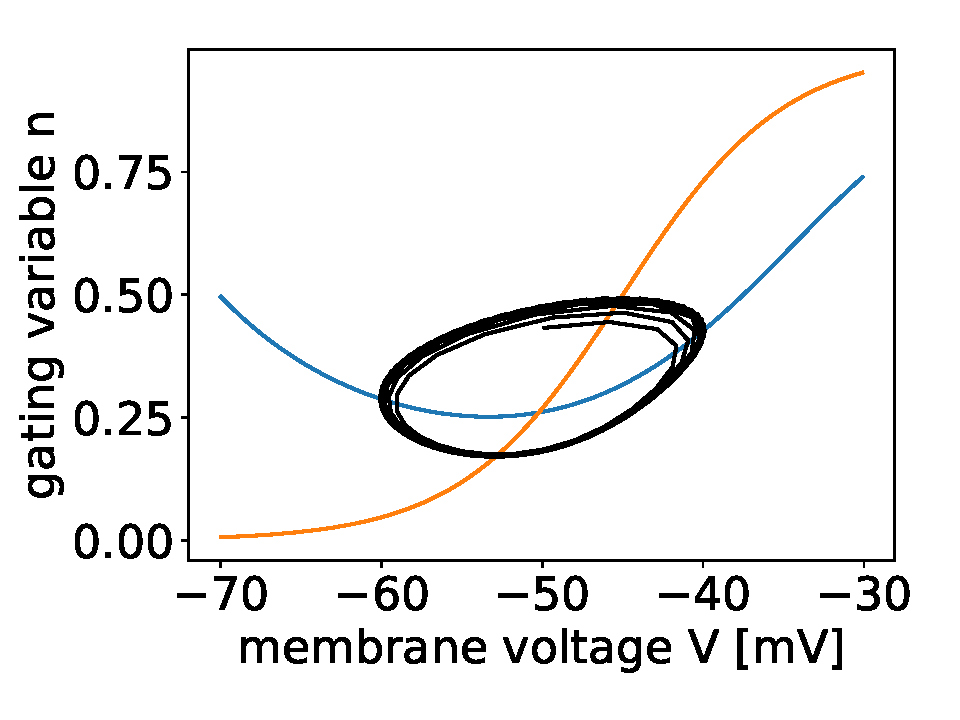
\includegraphics[scale=0.45]{inaprealanhopfunstablewn2black.pdf}} 
	\subfigure[]{	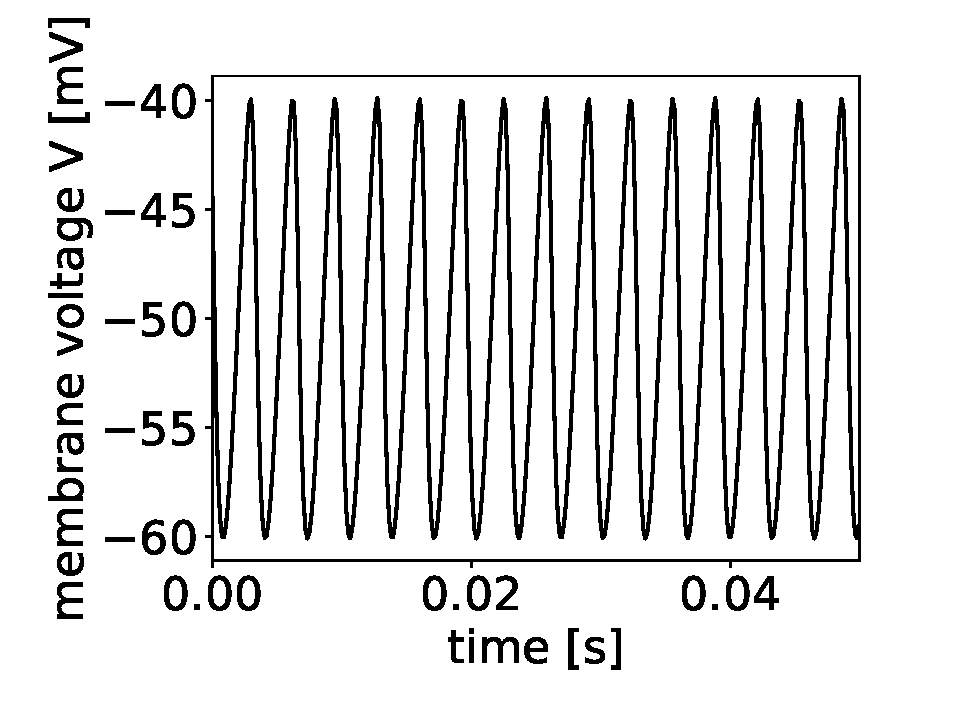
\includegraphics[scale=0.45]{inaprealanhopfunstablevtblack.pdf}}
	\caption{Evolution of the system on the unstable limit cycle. The left side shows the phase plane picture and on the right one can see the membrane voltage over time.}
	\label{unstable} 
\end{figure}
Due to the numerical impossibility to put the system exactly onto the unstable limit cycle, any time-forward simulation starting on the unstable cycle will eventually collapse into either stable configuration, as shown in figure \ref{divergent}.
\begin{figure}[H]
	\subfigure[]{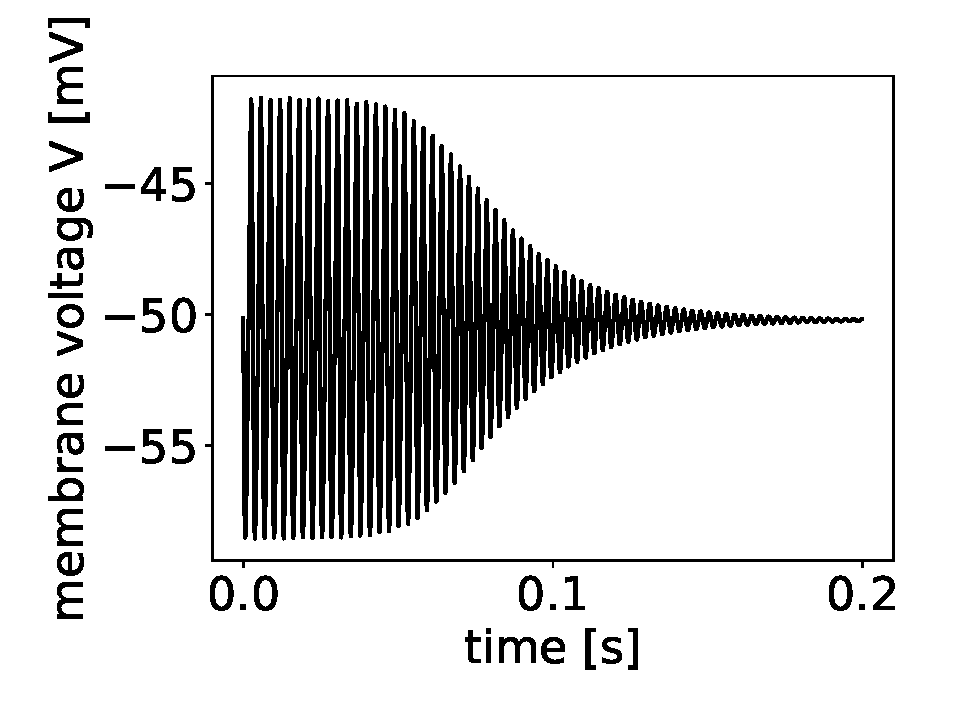
\includegraphics[scale=0.45]{inaprealanhopfnb2black.pdf}} 
	\subfigure[]{	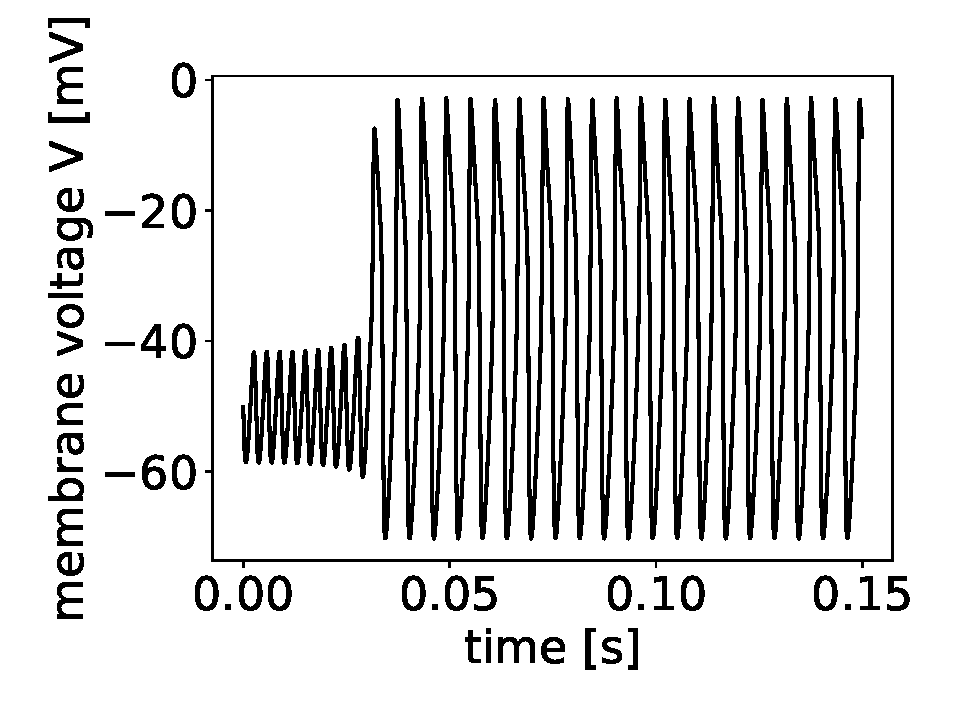
\includegraphics[scale=0.45]{inaprealanhopfunstable2black.pdf}}
	\caption{Evolution of the membrane voltage if the system is started near the unstable limit cycle. After a couple of circulations, the system quickly converges to a stable state.}
	\label{divergent} 
\end{figure}
\subsubsection{System with noise}
Considering that even in the noiseless system, the unstable limit cycle only lasts a few ms, it will not play any role in the noise-driven neuron. Therefore, the noise again just switches the system between spiking and resting state. The probability of each state can be influenced by tuning the bias current $I$, as can be seen in figure \ref{ahnoise}.
\begin{figure}[H]
	\subfigure[]{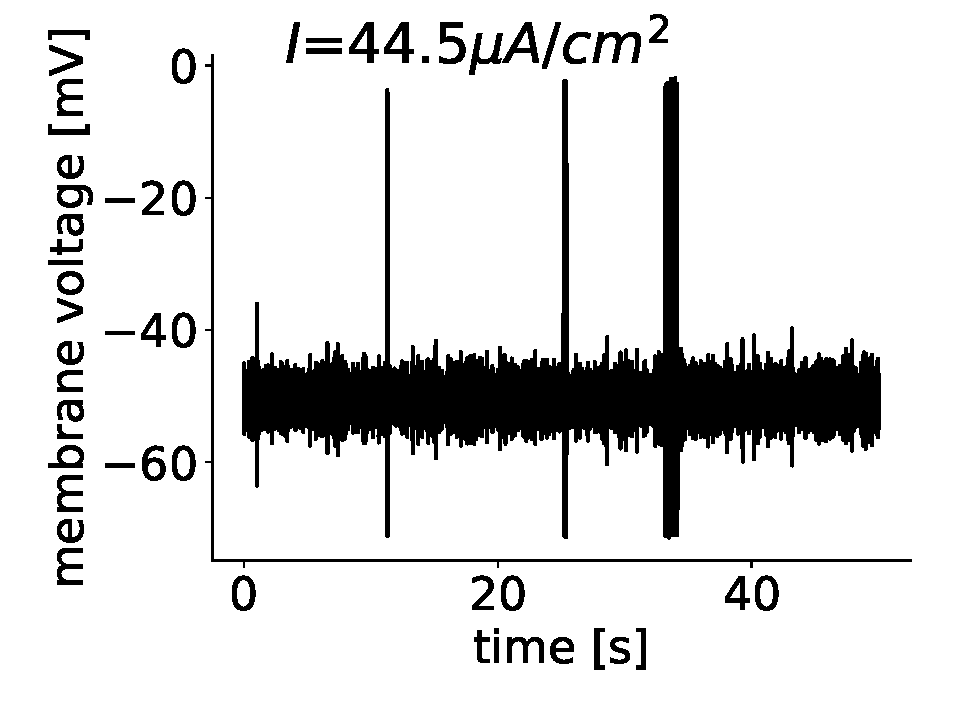
\includegraphics[scale=0.45]{realstateanhopf45full.pdf}} 
	\subfigure[]{	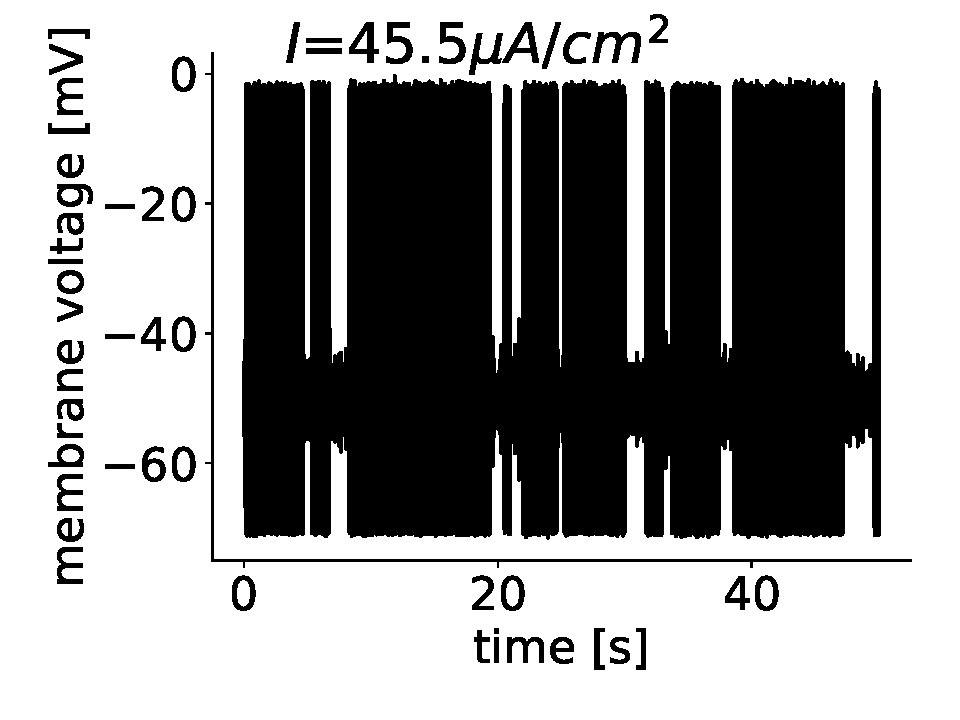
\includegraphics[scale=0.45]{realstateanhopf55full.pdf}}\\	\subfigure[]{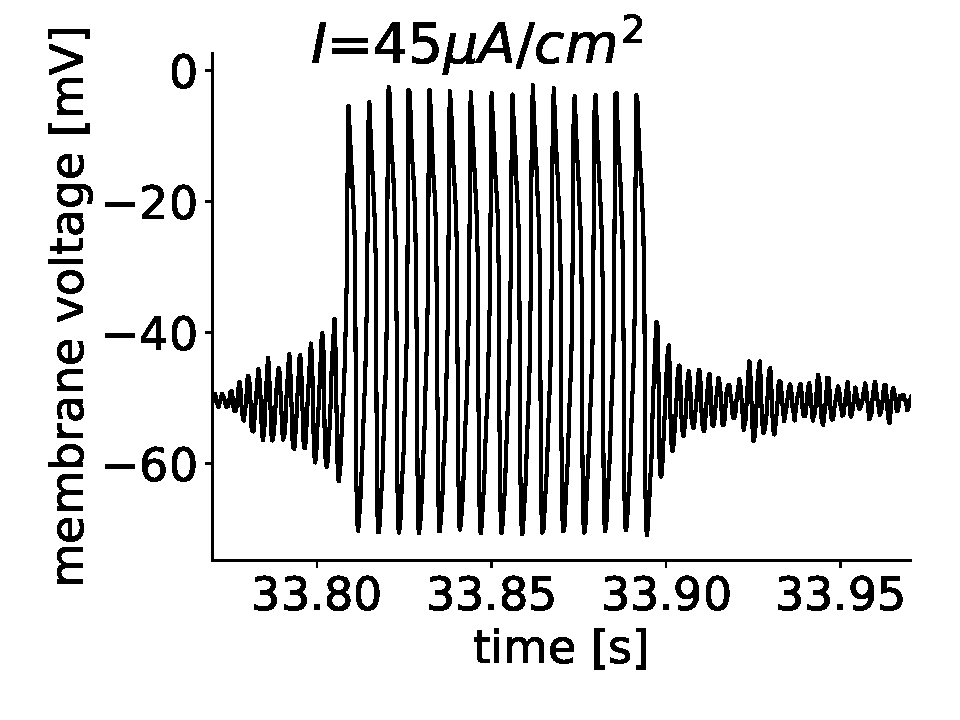
\includegraphics[scale=0.45]{realstateanhopf5sh3.pdf}} 
	\subfigure[]{	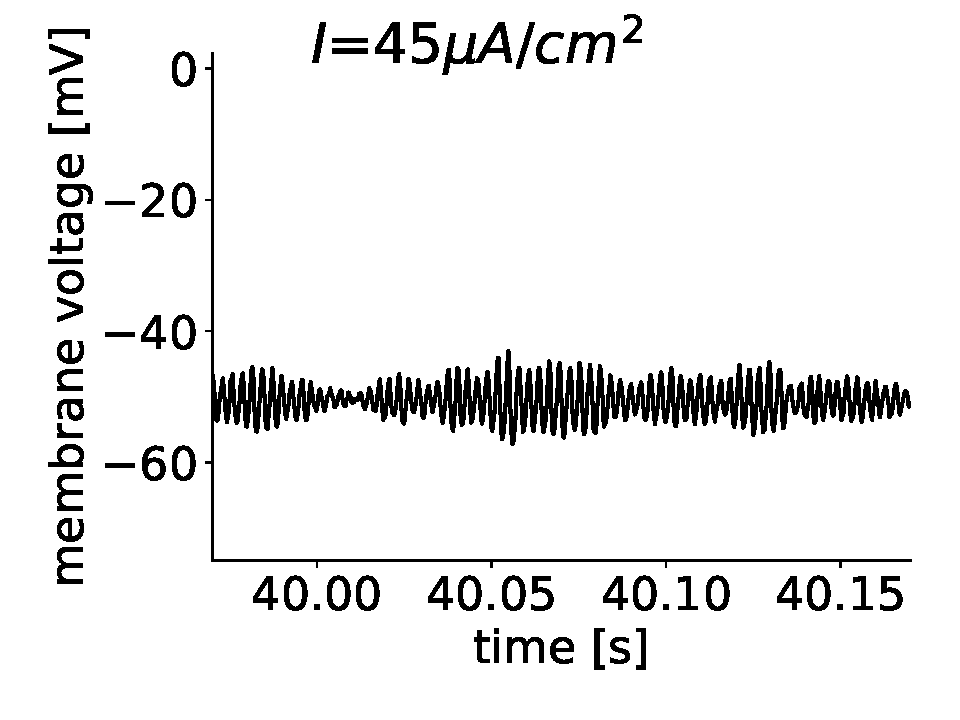
\includegraphics[scale=0.45]{realstateanhopf52sh.pdf}}
	\caption{Behavior of the membrane voltage for constant noise and changing bias current $I$ at $D=0.3$. On the bottom, one can see the behavior of the system with a higher time resolution. The small oscillations near equilibrum in (d) are subthreshold oscillations.}
	\label{ahnoise} 
\end{figure}
Over a range of $1\mu A/cm^2$, the neuron switches from barely spiking to basically only spiking. Due to the oscillatory properties of the system, small disturbances suffice to induce a change of state, if they occur at the right moment, as can be seen in 13 (c): Even though the state vector should be attracted to the stable focus, appropriate noise can slowly increase the amplitude of rotation until the spiking limit cycle is reached. In connection to this there exists another interesting phenomenon which is visible in (d): If the pulse amplitude is too small to make the neuron spike, it oscillates back to the focus with a high frequency. These subthreshold oscillations are a general characteristic of neurons with oscillatory potentials.
\subsection{Rinzel model}
The last model is a two-dimensional approximation of the Hodgkin-Huxley model, proposed by Rinzel in 1985 \cite{rinzel}. By assuming instantaneous $Na^+$ dynamics and expressing the two gating variables $h$ and $n$ by a single recovery variable $W$, Rinzel got the following model:
\begin{align*}
C\dot{V}&=I-g_{Na}m_\infty^3(V)(1-W)(V-E_{Na})-g_K(W/S)^4(V-E_K)-g_L(V-E_L)\\
\dot{W}&=\left[W_\infty(V)-W\right]/\tau(V)
\end{align*}
It has to be noted that for our simulations, white gaussian noise with intensity $D$ was added to the first equation.
However, the notation is almost similar to he $I_{na,p}+I_K$ model: $I$ denotes again the bias current, $C$ the capacitance, $V$ the membrane voltage, $g_i$ are conductances, $E_i$ the Nernst equilibrium potentials and $m_{\infty}$ the activation variable of the instantaneous $Na^+$ current. Inactivation of $Na^+$ and activation of $K^+$ are both governed by $W$. Its steady-state activation function $W_\infty$ is a linear combination of $n_\infty$ and $h_\infty$
\begin{align*}
W_\infty(V)=S\left(n_\infty(V)+S\left[1-h_\infty(V)\right]\right)/(1+S^2)\end{align*}
and $\tau$ comes from averaging the time constants of the gating variables
\begin{align*}
\tau(V)=\frac{5\exp[-(V+10)^2/55^2 ]+1}{3.82}
\end{align*}
The parameters were taken from the original Hodgkin-Huxley model:\\\\
$C=1$ , $g_L=0.3$ , $E_L=10$ , $g_{Na}=120$ , $E_{Na}=115$ , $g_K=36$ , $E_K=12$.\\\\
$S$ can be obtained from the resting values of $h$ and $n$
\begin{align*}
S=\frac{(1-h_\infty(0))}{n_\infty(0)}=1.27,
\end{align*}
and
\begin{align*}
k_\infty=\frac{\alpha_k}{\alpha_k+\beta_k}
\end{align*}
with
\begin{align*}
\alpha_n(V)&=0.01\frac{10-V}{\exp\left(\frac{10-V}{10}\right)-1}
&\beta_n(V)&=0.125\exp\left(\frac{-V}{80}\right)\\
\alpha_m(V)&=0.1\frac{25-V}{\exp\left(\frac{25-V}{10}\right)-1}
&\beta_m(V)&=4\exp\left(\frac{-V}{18}\right)\\
\alpha_h(V)&=0.07\exp\left(\frac{-V}{20}\right)
&\beta_h(V)&=\frac{1}{\exp\left(\frac{30-V}{10}\right)+1}
\end{align*}

\subsubsection{System without noise}
The first step in the phase plane analysis would again be determining the nullclines. Unfortunately, the variable $W$ not only appears linearly, but also in 4th power. This makes it analytically difficult to find a simple equation for the nullclines. Therefore, the nullclines were determined numerically:
\begin{figure}[H]
	\centering
	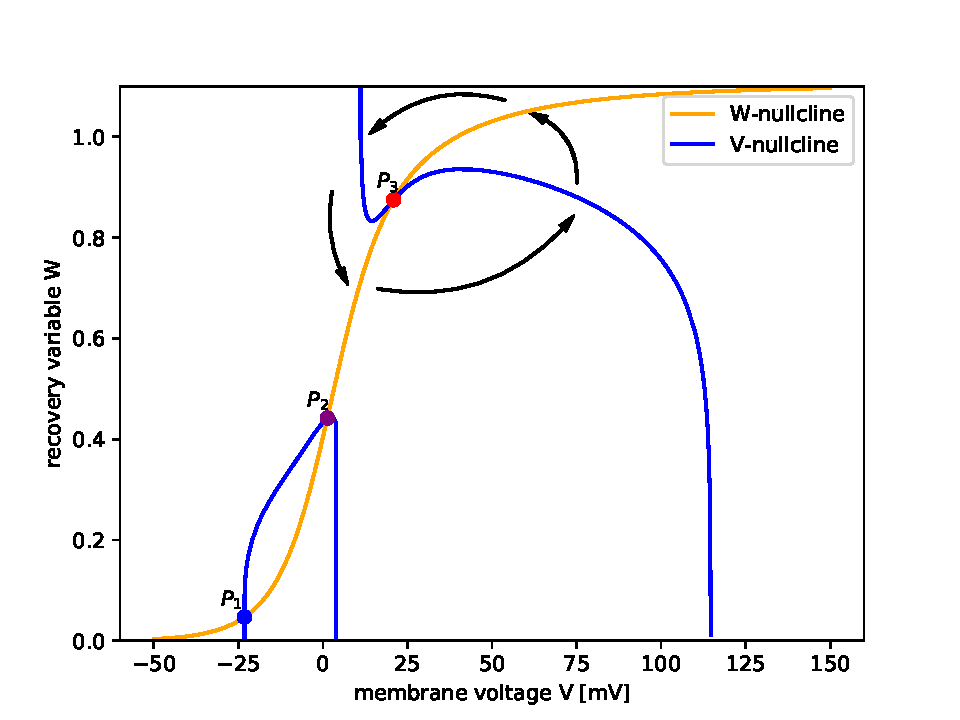
\includegraphics[scale=0.5]{rinzelclinesarrowwp.pdf}\caption{Nullclines of the Rinzel model with $I=-10$. The arrows indicate the direction of motion in the different regions.}
	\label{rinzelnc}
\end{figure}
Considering that this model is not a genuine two-dimensional neuron model, but just the result of a couple of simplifications carried out on the Hodgkin-Huxley model, the phase plane image can be understood as the 2-D projection of the 4-dimensional Hodgkin-Huxley model. Therefore, it comes as no surprise that the nullclines take on a more complex shape, consisting of a hill and an n-shaped part, both separated by a singularity at $V=10\text{mV}$. However, this does not change the fact that there are still 4 regions of different directions of motion, which are marked by arrows in figure \ref{rinzelnc}. \\
The numerical evaluation of the Jacobian matrix yields:
\begin{align*}
\lambda_+(P_1)&\approx-0.3 & \lambda_-(P_1)&\approx-0.7\\
\lambda_+(P_2)&\approx 0.5& \lambda_-(P_2)&\approx -1.4\\
\lambda_+(P_3)&\approx 6.3& \lambda_-(P_3)&\approx 0.5
\end{align*}
This means that there is a stable node at $P_1$, a saddle at $P_2$ and an unstable node at $P_3$. Upon increase of $I$, the hill will move downwards, eventually leading to a merger of $P_1$ and $P_2$ at $I\approx -5.91$ when the system undergoes a saddle-node bifurcation and is no longer in the bistable regime.\\
When it is in the bistable regime, there are two sets of initial conditions, leading either to quiescence or repetitive firing as shown in figure \ref{subfigrinzel}.
\begin{figure}[H]
	\subfigure[]{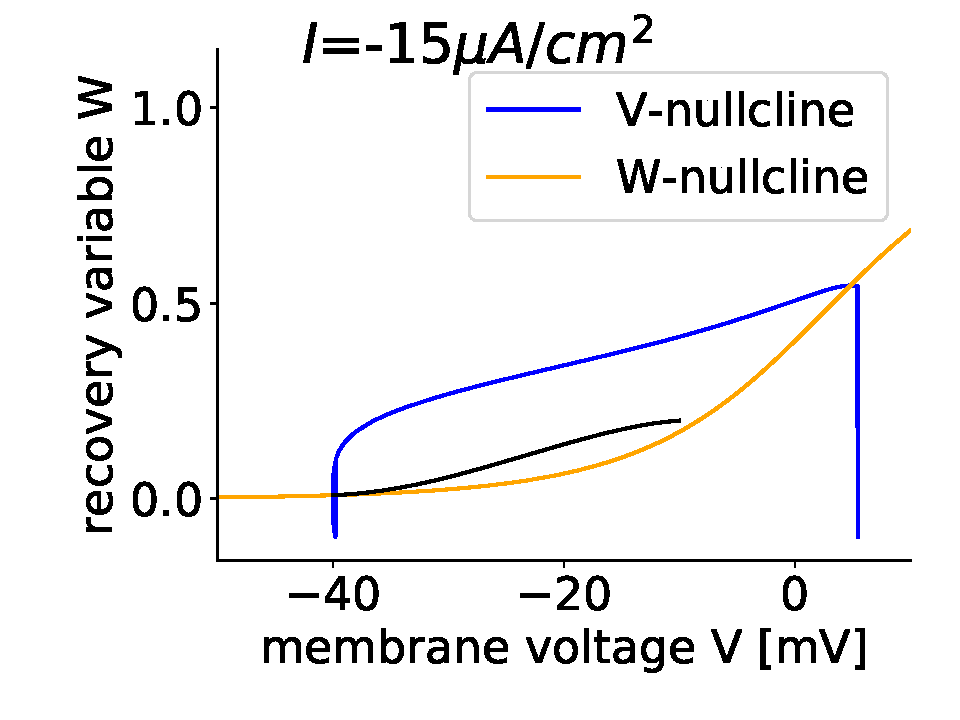
\includegraphics[scale=0.45]{realstatedetrinzelpnb2wnblack.pdf}} 
	\subfigure[]{	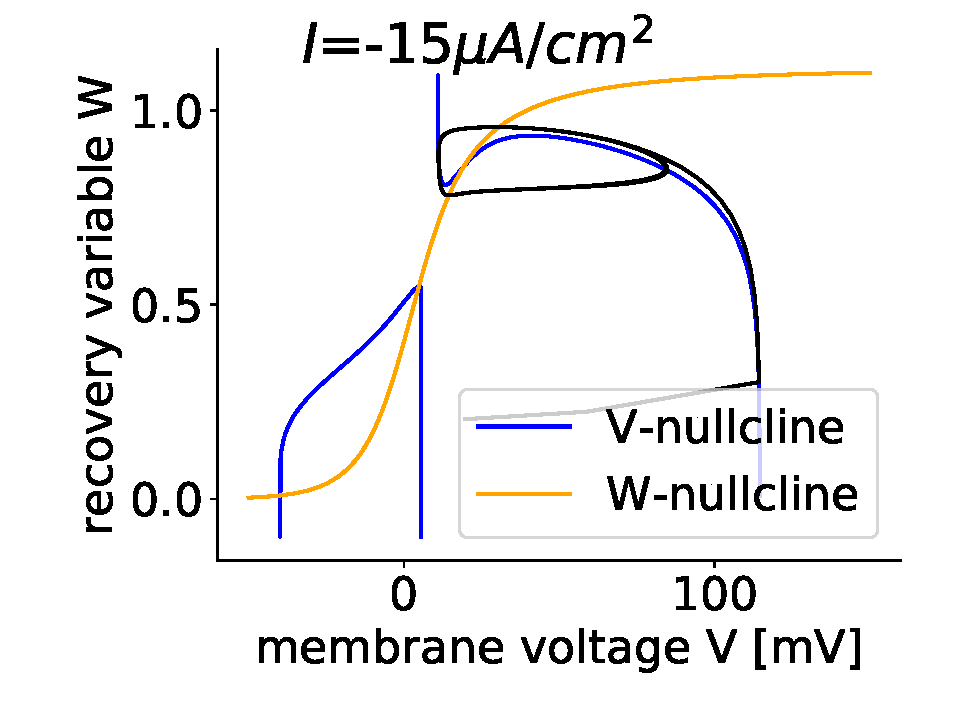
\includegraphics[scale=0.45]{realstatedetrinzelpnbwnblack.pdf}}\\	\subfigure[]{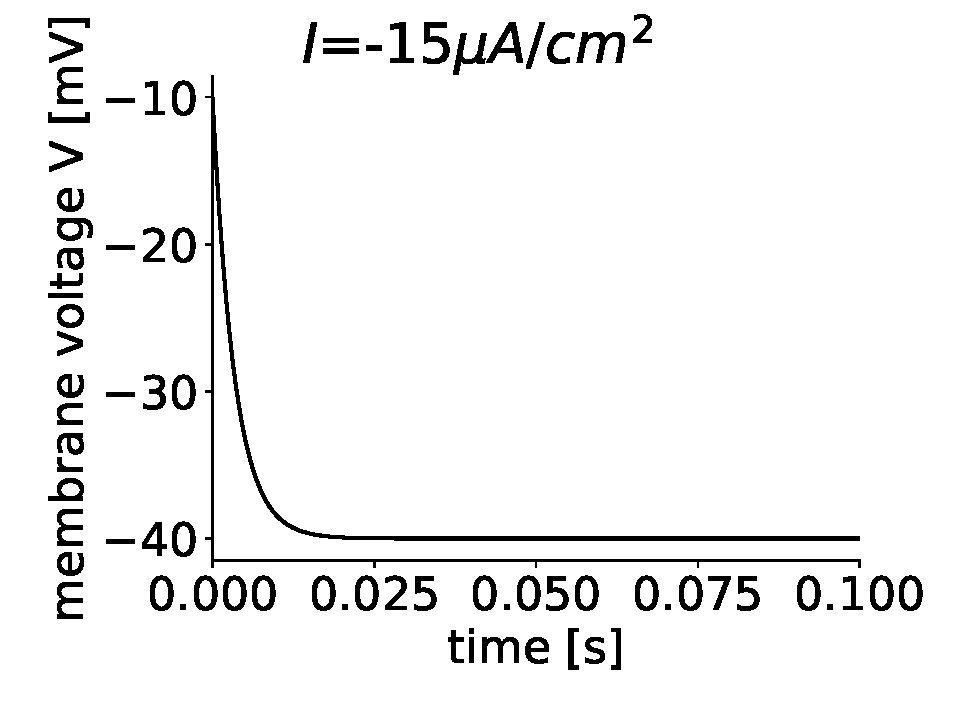
\includegraphics[scale=0.45]{realstatedetrinzelpnb2.pdf}} 
	\subfigure[]{	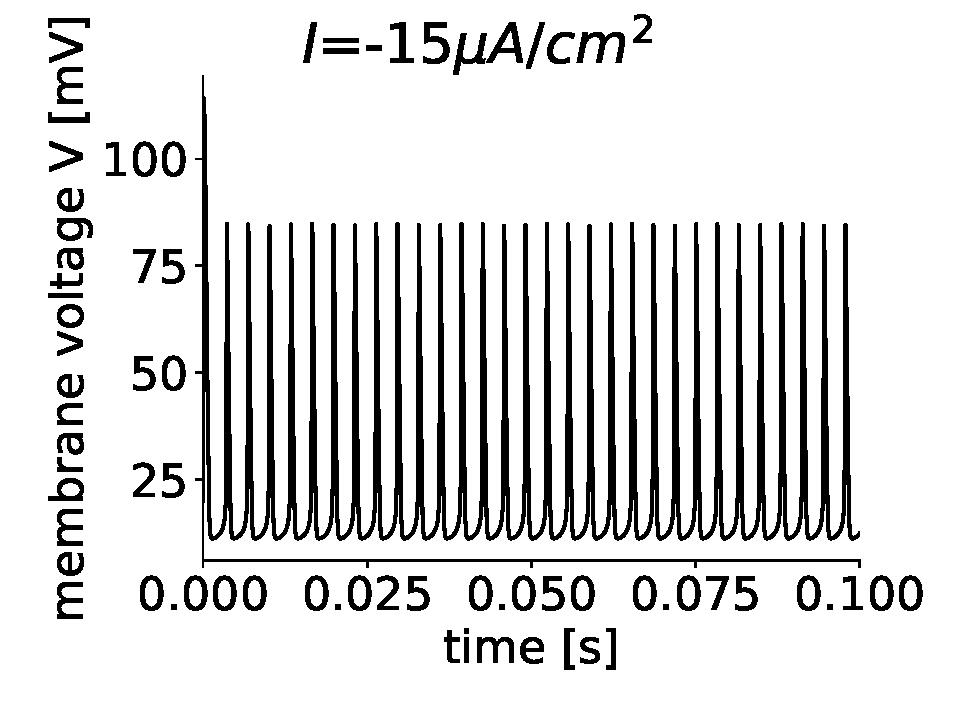
\includegraphics[scale=0.45]{realstatedetrinzelpnb.pdf}}
	\caption{Evolution of the phase vector (first row) and the membrane voltage over time (second row). The left side shows the evolution of the system with resting ICs, and on the right one can see the behavior under spiking ICs.}
	\label{subfigrinzel} 
\end{figure}
Apparently, it is only a matter of a couple tens of microseconds to reach a stable configuration: the system converges exponentially to the stable equilibrium or after an initial spike, it goes around on the spiking limit cycle, respectively.\\
The two sets of initial conditions can once again be distinguished by letting the system evolve without noise from different starting points:
\begin{figure}[H]
	\hspace*{-0.5cm}
	\subfigure[]{	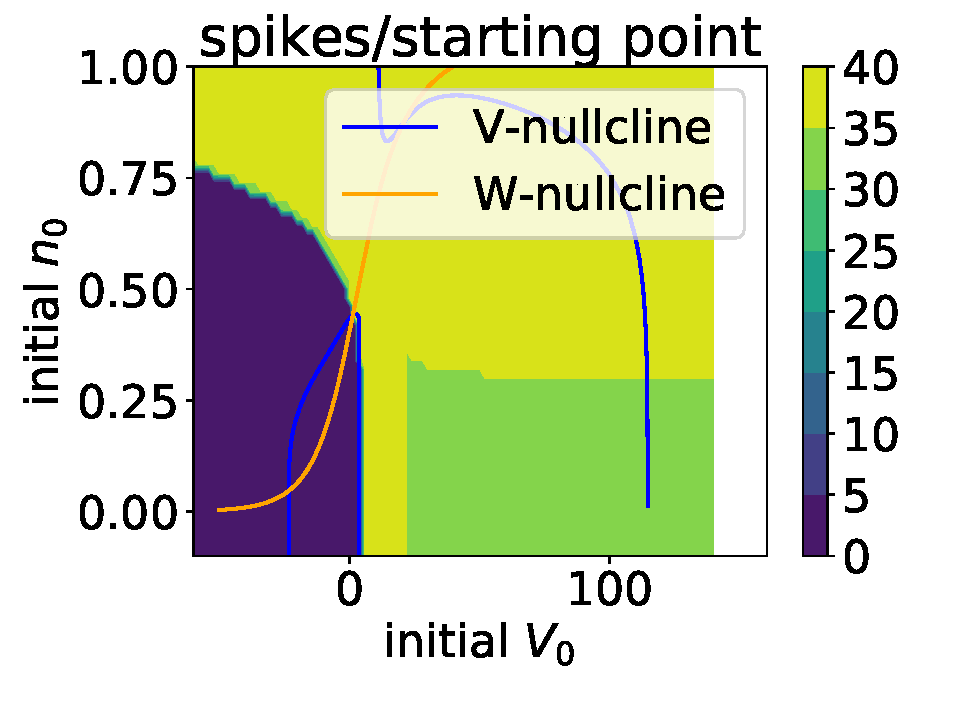
\includegraphics[scale=0.5]{contourrinzela12shalt3.pdf}}
	\subfigure[]{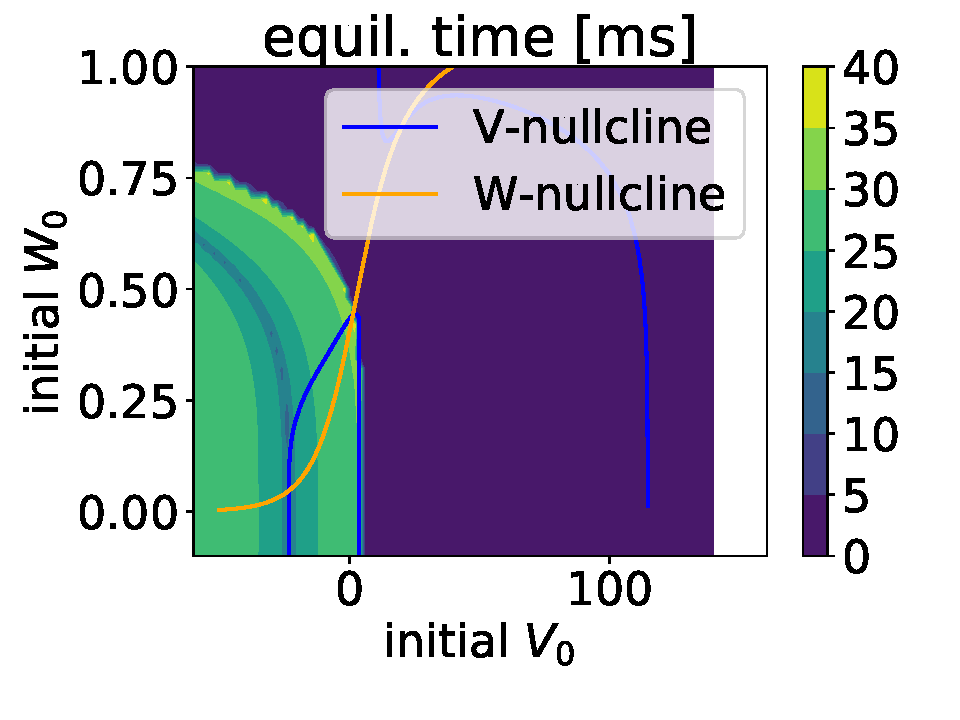
\includegraphics[scale=0.5]{contourrinzela12time.pdf}}
	
	\caption{Phase plane image of the neuron model with $I=-10$ and no noise. Each point represents a specific combination of starting parameters. The left plot shows the number of spikes over a short period of time and for the right picture, the equilibration times for both states were measured. Irregularities arise from the finite resolution of the $V_0$-$n_0$-lattice.}
	\label{twodomrinzel}
\end{figure}
Even though the nullclines have a more complex shape, the sets of initial conditions are again separated by a single line.
Interestingly, the plots in figure \ref{twodomrinzel} look inverse to each other. This means that the firing state is reached much faster than the resting state, almost independent of the starting point. Similarly to the $I_{Na,p}+I_K$-model, the border goes, as expected, through the saddle point.
\subsubsection{System with noise}
Now that the model has been understood in the phase plane, the influence of noise can be investigated.
\begin{figure}[H]
	\subfigure[]{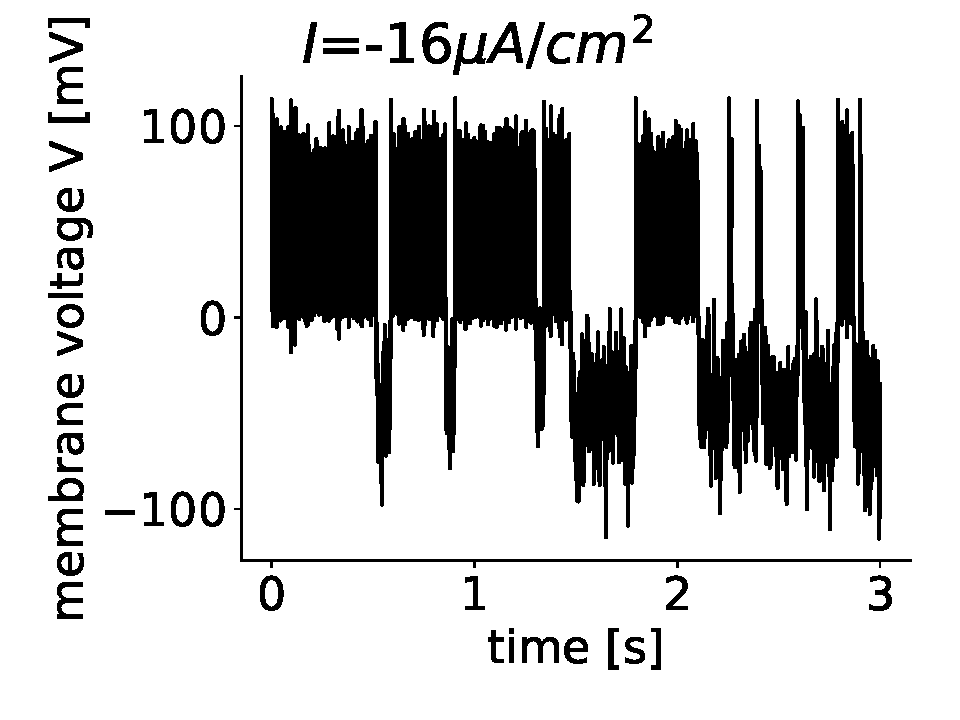
\includegraphics[scale=0.45]{realstatedetrinzel16100.pdf}} 
	\subfigure[]{	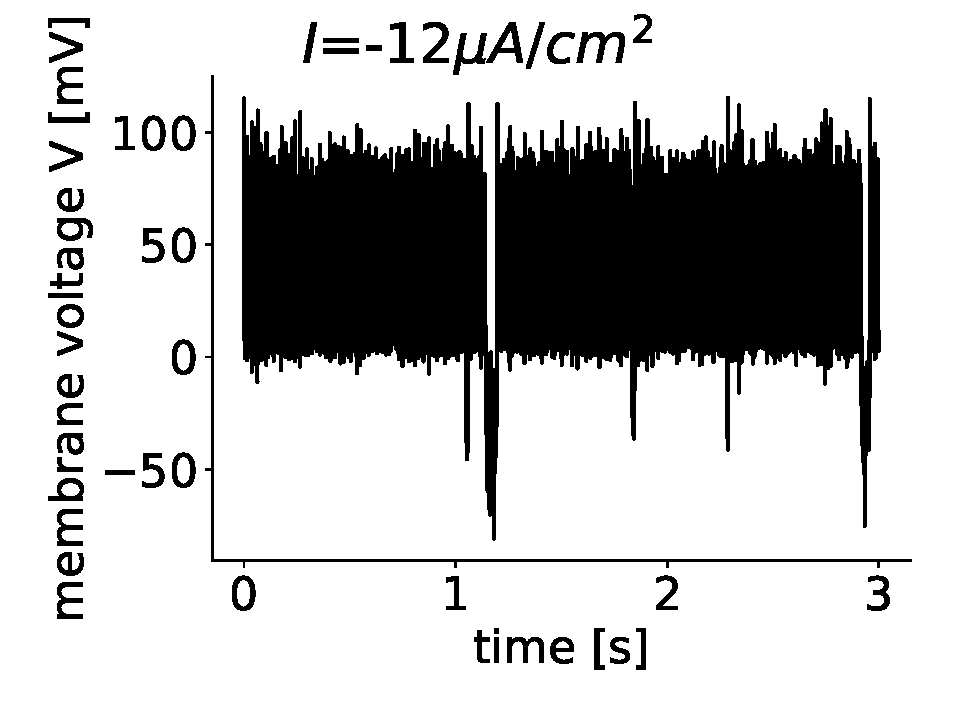
\includegraphics[scale=0.45]{realstatedetrinzel12100.pdf}}\\	\subfigure[]{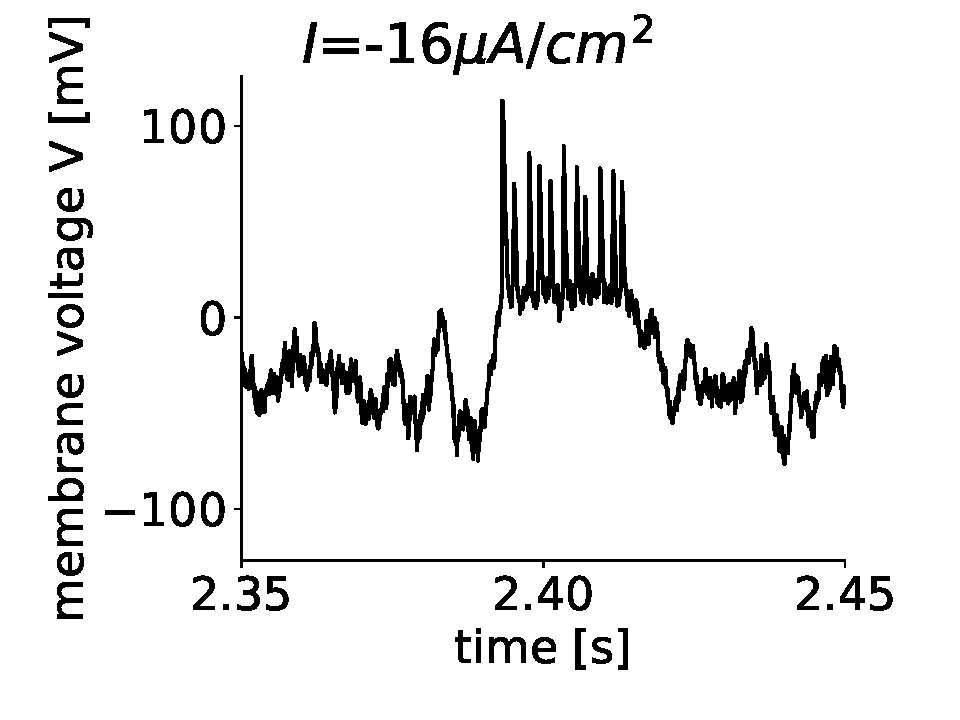
\includegraphics[scale=0.45]{realstatedetrinzel16100sh2.pdf}} 
	\subfigure[]{	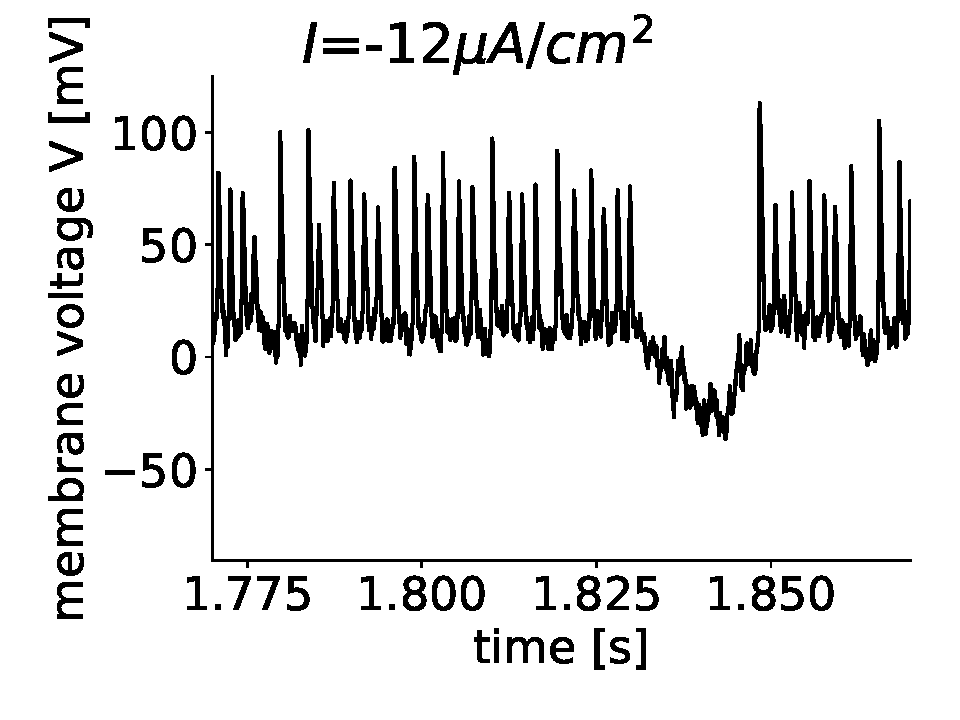
\includegraphics[scale=0.45]{realstatedetrinzel12100sh.pdf}}
	\caption{Behavior of the membrane voltage for constant noise and changing bias current $I$ at $D=100$. On the bottom, one can see the behavior of the system with a higher time resolution.}
	\label{rinzelnoise} 
\end{figure}
Here, too, the bias current $I$ is the parameter that controls whether resting or spiking state is preferred. At intermediate $I$, the neuron fires irregularly and the noise has a high impact on its behavior. At high bias currents, the neuron barely goes into the resting state, and even that only for a short period of time before going back to tonic spiking. The major impact of noise in this regime lies in the modulation of firing rate and spike height, clearly visible in \ref{rinzelnoise} (d).
\subsection{Quantities of interest}
\subsubsection{System without signal}
In the context of Brownian Motion, there were two characteristic quantities: the ensemble of particles moves with a mean velocity
\begin{equation}
\left\langle v\right\rangle =\lim_{t\rightarrow\infty}\frac{\left\langle x(t)-x(0) \right\rangle}{t}
\end{equation}
and is subject to a diffusive spread around this average flow that can be described by the effective diffusion coefficient
\begin{equation}
D_{eff}=\lim_{t\rightarrow\infty}\frac{\left\langle x^2(t) \right\rangle-\left\langle x(t)\right\rangle ^2}{2t}
\end{equation}
In the context of neuron models, similar quantities can be defined. The most important event with regard to signal transmission is the generation of a spike. Therefore, it is often useful to approximate the voltage curve by a spike train where every spike is assumed to be a Dirac-delta function,
\begin{equation}
x(t)=\sum_{i}\delta(t-t_i)
\end{equation}
The most relevant quantity is the spike count $N(t)$ which describes the number of spikes fired after a time $t$. This can be easily found by integrating the spike train over time:
\begin{equation}
N(t)=\int_{0}^{t}dt'x(t')=\sum_{t_i<t} 1
\end{equation}
Instead of the mean velocity, one can ask for the average firing rate
\begin{equation}
\left\langle v\right\rangle =\lim_{t\rightarrow\infty}\frac{\left\langle N(t) \right\rangle}{t}
\end{equation} 
and the diffusive spread of the spike count
\begin{equation}
D_{eff}=\lim_{t\rightarrow\infty}\frac{\left\langle N^2(t) \right\rangle-\left\langle N(t)\right\rangle ^2}{2t}
\end{equation}
A more common way to measure spiking variability in neurons is the Fano factor:
\begin{align*}
F=\frac{\left\langle \Delta N^2(t) \right\rangle}{\left\langle N(t)\right\rangle}=\frac{2D_{eff}}{\langle v\rangle}
\end{align*}
\subsubsection{System with signal}
When bistable neurons are subjected to a periodic stimulus, they should change their firing pattern accordingly. This is best visible in the power spectrum of the spike train, 
\begin{equation}
S(f)=\lim_{T\rightarrow\infty}\frac{\langle|\tilde{x}|^2\rangle}{T}
\end{equation}
%\subsection{Giant Diffusion}
%The term \glqq Giant Diffusion \grqq is short for \textit{Giant Enhancement of (thermal) diffusion} which was first observed around the turn of the millennium for Brownian Particles in a tilted periodic potential\cite{td}\cite{ga}\cite{dit}\cite{gd}. In general, these particles exhibit two stable velocity states. They can be \glqq trapped\grqq in a potential minimum - this is referred to as the \textit{locked state} - or they can be in the \textit{running state}. A particle gets into the running state if it has managed to overcome a hill and the frictional loss is low enough so that it is able to pass the adjacent hills as well. In the case of large friction or a strongly tilted potential, however, only one of these two states is present. If the potential is tilted in such a way that both states exist and the probabilities to be in either state are similar, many switchings between the states will occur. In the weak-noise-limit, half of the particles will be mainly in the locked state, while for the others the running state prevails. This behavior leads to diverging diffusion coefficients known as Giant Diffusion.
%\subsection{Giant diffusion of Brownian Particles}
%First observed by the botanist Robert Brown in 1828\cite{bm}, the term \textit{Brownian Motion} describes the irregular movement of particles in a viscous medium, whose apparently random changes of direction are caused by collisions with smaller particles or molecules.
%\\
%Ordinary Brownian Motion obeys a simple linear Langevin-equation:
%\begin{align*}
%\text{m}\dot{v}=-\lambda v+\xi(t)
%\end{align*}
%The evolution of the velocity $v$ of the particle is affected by a linear friction term with coefficient $\lambda$ and a random force $\xi(t)$. \\
%\\ 
%In the following, two different systems with Brownian Motion dynamics exhibiting Giant Diffusion are presented. These were the motivation for my research on bursting neuron models.
%\subsubsection{Active Brownian Particles}
%Active Brownian Motion can be observed on small organisms, like bacteria or cells, which are able to move on their own. In order to model the behaviour of such an object, a more general friction term needs to be introduced into the Langevin-equation:
%\begin{align*}
%\dot{v}=-f(v)+\xi(t)
%\end{align*}
%Here, the noise was assumed to be additive and the mass was omitted due to clarity.
%An accurate description of the self-propulsion can be accomplished by choosing the function $f$ in such a way that it attains negative values at small velocities and becomes greater than zero at large speed. Thus, at small velocities the particle will accelerate and with increasing velocity, regular friction will start to affect its motion.
%\\
%A system like this was studied by Lindner and Nicola in 2008\cite{abp}. They chose a cubic function for the friction term, $f(v)=v-v^3+F$, allowing them to write the equation of motion in terms of a quartic velocity potential $U(v)$:
%\begin{equation}
%\dot{v}=-U'(v)+\xi(t)
%\end{equation}
%with $U(v)=\frac{1}{4}v^4-\frac{1}{2}v^2-Fv$.
%\begin{figure}[H]
%	\centering
%	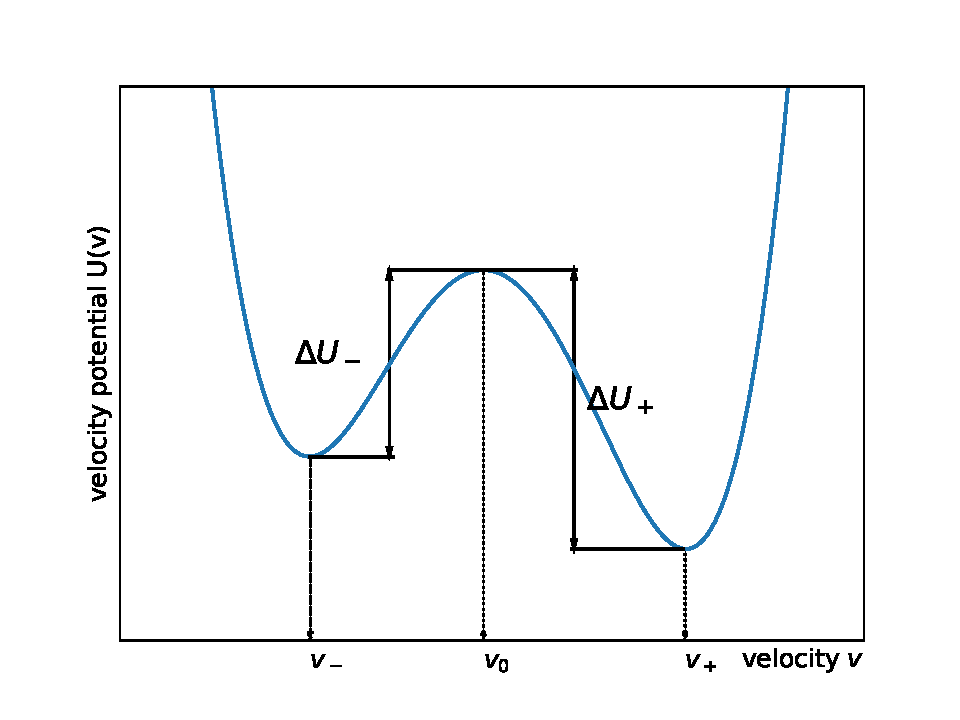
\includegraphics[scale=1]{velpot.pdf} 
%	\caption{tilted velocity potential of an Active Brownian Particle}
%	\label{velpot}
%\end{figure}
%This potential shows two minima at $v_\pm$, representing the stable velocity states \glqq forwards\grqq and \glqq backwards\grqq, and a maximum at $v_0$. In order to transition from $v_\pm$ into the other state, the particle needs to overcome a barrier of height $\Delta U\pm$.  
%\\
%Their simulations revealed a certain region of bias forces $F$, in which giant diffusion occurred.
%\begin{figure}[H]
%	\centering
%	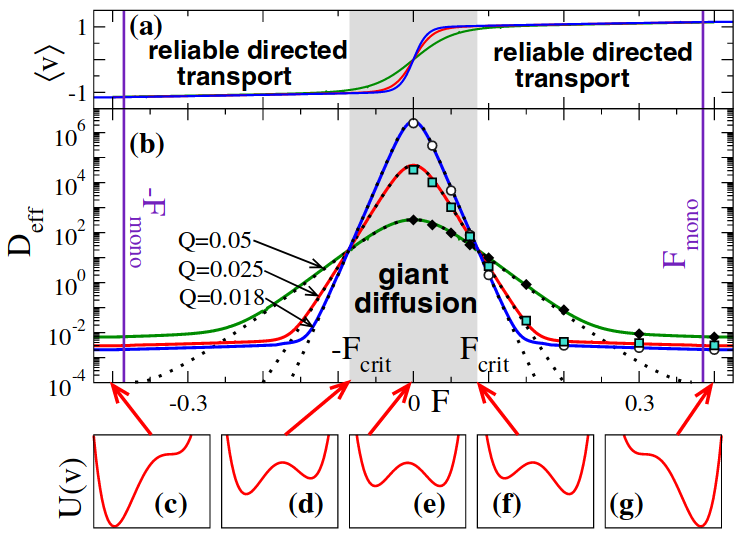
\includegraphics[scale=0.5]{mess08.png}\caption{Simulation of velocity and effective diffusion coefficient for Active Brownian Particles underlying a tilted velocity potential,taken from \cite{abp}}
%	\label{abpsim}
%\end{figure}
%Inside this region, the diffusion coefficients increase with decreasing noise intensity, while they decrease outside of this region. In other words, in the weak noise limit, the diffusion coefficients diverge in the critical region and vanish outside of it. The critical force lies at the border of this region and emerges from the intersection points of the diffusion coefficients for different noise levels. A simple criterion could be found for these intersection points: at the critical force, one potential barrier is twice as high as the other potential barrier. 
%Furthermore, it is remarkable that the reliable directed transport which takes place outside of the critical region appears much earlier than the monostability of the velocity potential, which is a obviously only a primitive criterion for reliable transport in one direction. 
%The mean velocity displays a more regular behavior. It is almost constant at a value less than zero up to small negative forces, then undergoes a sharp increase to a positive value and barely changes afterwards. They intersect as well, approximately at the position where the diffusion coefficient gets maximal.
%\subsubsection{Regular Brownian Particles in a tilted periodic potential}
%On their own, ordinary Brownian Particles do not exhibit bistable velocity dynamics which may lead to giant diffusion. But as mentioned before, this can be done by adding a periodic potential to the equation of motion:
%\begin{equation}
%\dot{v}=-\gamma v-U'(x)+\sqrt{2\gamma kT}\xi(t)
%\end{equation}
%with $U(x)=-Fx-d\cos(x)$. This system was discussed with respect to giant diffusion in a paper by Lindner and Sokolov from 2016\cite{bpp}. Now, in contrast to the Active Brownian Particle, the evolution of the system is not governed by a velocity potential, but by a spatial potential:
%\begin{figure}[H]
%	\subfigure[]{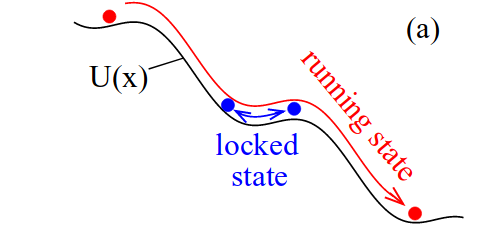
\includegraphics[width=0.5\textwidth]{veldynupper.png}} 
%	\subfigure[]{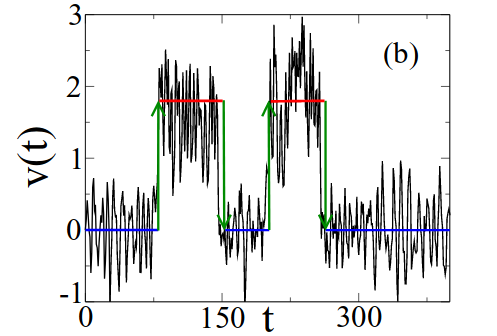
\includegraphics[width=0.5\textwidth]{veldynlower.png}} 
%	\caption{Figure (a) visualizes the motion of a Brownian Particle in a periodic potential, on the right one can see the bistable velocity dynamics. The oscillations thereby arise from local extrema of the potential.}
%	\label{veldyn} 
%\end{figure}
%Also for the Brownian Particles in a cosine potential, there was a finite range of bias forces, for which giant diffusion could be observed:
%\begin{figure}[H]
%	\centering
%	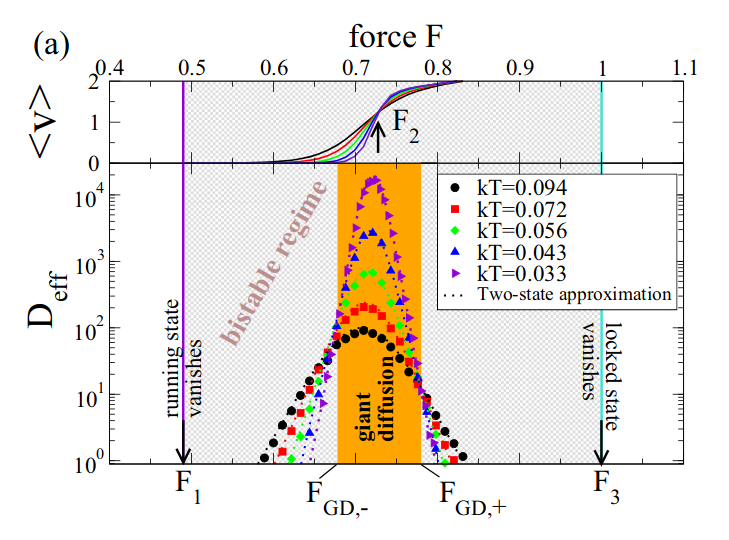
\includegraphics[scale=0.5]{nbpsim1.png}\caption{Simulation of velocity and effective diffusion coefficient for Brownian Particles in a tilted periodic potential,taken from \cite{bpp}}
%	\label{anbpsim}
%\end{figure}
%Again, all curves of the diffusion coefficient intersect at two points and diverge in between those points for decreasing noise intensities while going to zero on the outside and the velocity curves intersect approximately at the maximum of the diffusion coefficient. And also here the region of giant diffusion is much smaller than the range of bias forces, where both states coexist. Two other variables that help characterize the system are the transition rates between the states, that is from the locked to the running state and vice versa. Even though there didn't exist actual potential barriers, these turned out to obey an Arrhenius or Kramers law, respectively, as can be seen from an Arrhenius plot:
%\begin{figure}[H]
%	\centering
%	\includegraphics[scale=0.5]{kramerfit.png}\caption{Fits of the transition rates with both an Arrhenius and a Kramers law, taken from \cite{bpp}}
%	\label{bparr}
%\end{figure}
%In this example, the Arrhenius fit as well as the Kramers fit yield good agreements with the data. From these fits one can extract effective potential barriers. The relation found for the potential barriers of the Active Brownian Particle can be tested by plotting the effective barriers and twice their value:
%\begin{figure}[H]	\includegraphics[scale=0.5]{barrierplot.png}\caption{Plot of the effective potential barriers. The dotted curves are simply twice the solid curves of the same color. This plot is taken from \cite{bpp}}
%\end{figure}
%The plot shows that the points where one potential barrier equals twice the other roughly correspond to the critical forces, so the criterion applies as well to this case, where no potential barriers were present and only effective barriers could be calculated.
%\subsection{Two-state theory}\label{tst}
%In the case of low noise intensity, the transition times between the locked state and the running state will be much shorter than the periods of time that the particle stays in one of the two states. That is why it is practical to describe the behavior of the system in this regime with a two-state model. The following derivation applies to the Brownian Particle in a tilted periodic potential. The transition rates are assumed to obey an Arrhenius law:
%\begin{align*}
%r_{\pm}=r_{0,\pm}\exp\left(-\frac{\Delta U_{\pm}}{D}\right)
%\end{align*}
%where $r_-$ denotes the transition rate from locked to running state, and $r_+$ the rate for the other transition. $\Delta U_{\pm}$ is the corresponding potential barrier and $D$ the noise intensity. The effective diffusion coefficient can be calculated from the velocity $v_0$ in the running state and the transition rates: 
%\begin{align*}
%D_{\text{eff}}=\frac{v_0^2 r_+r_-}{(r_++r_-)^3}
%\end{align*}
%The first task is to find the intersection points of the diffusion coefficients. At these points, the diffusion coefficients become independent of the noise intensity.
%It is
%\begin{align*}
%D_{\text{eff}}&=\frac{v_0^2r_{0,+}r_{0,-}\exp\left(-\frac{\Delta U_++\Delta U_-}{D}\right)}{\left[r_{0,+}\exp(\frac{-\Delta U_+}{D})+r_{0,-}\exp\left(\frac{-\Delta U_-}{D}\right)\right]^3}\\&=\frac{v_0^2r_{0,+}r_{0,-}}{\left[r_{0,+}\exp\left(-\frac{3\Delta U_+-\Delta U_+-\Delta U_-}{3D}\right)+r_{0,-}\exp\left(-\frac{3\Delta U_--\Delta U_+ -\Delta U_-}{3D}\right)\right]^3}\\&=\frac{v_0^2r_{0,+}r_{0,-}}{\left[r_{0,+}\exp\left(-\frac{2\Delta U_+-\Delta U_-}{3D}\right)+r_{0,-}\exp\left(-\frac{2\Delta U_--\Delta U_+}{3D}\right)\right]^3}
%\end{align*}
%In the limes $D\rightarrow 0,\Delta U_+>U_-$ the first term in the denominator vanishes, resulting in:
%\begin{align*}
%D_{\text{eff}}=\frac{v_0^2r_{0,+}}{r_{0,-}^2}\exp\left(-\frac{\Delta U_+-2\Delta U_-}{D}\right)
%\end{align*}
%Under the assumption that the prefactors change slowly in comparison to the exponential function, the following condition arises:
%\begin{align*}
%\Delta U_+=2\Delta U_-
%\end{align*}
%Due to symmetry of the problem, the opposing case $D\rightarrow 0,\Delta U_+<U_-$ yields:
%\begin{align*}
%\Delta U_-=2\Delta U_+
%\end{align*}
%In both cases, one potential barrier is twice as high as the other one.\\
\subsection{Two-state theory}
Next, we will examine whether the Fano factor displays similar features in the weak noise limit. As 
\begin{align*}
F=\frac{2D_{\text{eff}}}{L\langle v\rangle}
\end{align*}
an expression for the average velocity is required to compute the Fano factor. Taking into account that the average velocity is zero when the particle is in the locked state, one finds the following formula for the total mean velocity:
\begin{align*}
\langle v\rangle=v_0\frac{r_-}{r_++r_-}
\end{align*}
Therefore
\begin{align*}
F=\frac{2v_0r_+}{(r_++r_-)^2}=\frac{2v_0r_{0,+}\exp\left(\frac{-\Delta U_+}{D}\right)}{\left(r_{0,+}\exp\left(\frac{-\Delta U_+}{D}\right)+r_{0,-}\exp\left(-\frac{\Delta U_-}{D}\right)\right)^2}
\end{align*}
In the limes $D\ll1$ there are again two solutions. For $\Delta U_+ > \Delta U_-$:
\begin{align*}
F=\frac{2v_0r_{0,+}}{r_{0,-}^2}\exp\left(-\frac{\Delta U_+-2\Delta U_-}{D}\right) \rightarrow \Delta U_+=2\Delta U_-
\end{align*}
as well as for $\Delta U_+ < \Delta U_-$:
\begin{align*}
F=\frac{2v_0}{r_{0,+}}\exp\left(-\frac{\Delta U_+-2\Delta U_+}{D}\right) \rightarrow \Delta U_+=0
\end{align*}
The intersection point for $\Delta U_+ > \Delta U_-$ stays the same while at the other critical point the potential barrier from running to locked state needs to vanish. As the latter condition violates the requirements for the application of the two-state theory - because only one state would exist in this case - the second intersection point can't be determined via this two-state model.
%\section{Giant diffusion in a bursting neuron model}
%\subsection{Brownian motion and neuronal models}
%Brownian motion in periodic potentials has numerous applications among which one can find superionic conduction, rotation of a dipole in a static field or the description of a Josephson Tunneling junction\cite{fpe}. However, apart from these mechanical examples, Brownian motion in periodic potentials is also suited to describe a bursting neuron. If one counts every time the particle crosses a hill as a spike, the running state can be associated with tonic firing and the locked state with a stable equilibrium point. Because of the random noise, transition between the states will occur and the sustained spiking will be eventually terminated so that there is only a finite number of spikes within each burst. The position of the Brownian Particle then corresponds to the spike count of the neuron and its velocity to the firing rate. Thus, based on the similarities to Brownian motion, we expect to find a weak noise behavior comparable to giant diffusion also in bursting neurons.
%\subsection{Neuronal bursting}
%Depending on its physiology and the properties of the stimulus, a neuron doesn't always fire a single spike. A series of multiple spikes in a short time interval that is followed by a period of quiescence is called a burst\cite{izi}. Typically, bursting results from the interplay between two subsystems: a fast subsystem, that is responsible for the generation0 of the spikes within a burst, and a slow subsystem that modulates the bursting pattern and eventually terminates sustained spiking. However, a bursting neuron model that implements these slow and fast dynamics would at least have to be three-dimensional, as there would be a variable for the membrane voltage as well as for the fast and slow oscillations. One way to realize a bursting two-dimensional model and to make use of the various methods of phase plane analysis is to introduce noise into the system. Considering that any neuron is subject to some kind of noise, this is a justified assumption and was even proposed by Izhikevich as a way to make two-dimensional neuronal models burst\cite{izi}.
%\subsection{The bursting neuron model}
\subsection{Numerical implementation}
The behavior of the two-dimensional neuron model can be investigated by conducting simulations with the parameters described above and evaluating the data in a couple different ways. The simulations were done by letting the system evolve almost freely with the only external influence being the white gaussian noise with intensity $D$. \\
In all of the computations, only a single neuron was simulated over a long period of time. When investigating an ergodic system, this procedure ensures that the results are independent of the initial conditions if the simulation time is long enough. Furthermore, an ensemble of neurons would need to be equilibrated before starting any measurements so that the obtained results would be correct. This equilibration time can be omitted now, which saves some computation time. \\
Mostly, the spike train was cut into 500 segments. Only for $D=0.25$, the number of neurons was set to 50 so that there would be a higher number of transitions in a single voltage curve. In all cases, the timestep was 0.5 $\mu$s. The total measurement time for each spike train ranged from $5\cdot10^5$ s for high noise intensities to $2\cdot 10^6$ s for the lowest noise intensities, yielding lengths between $10^3$ and $4\cdot10^4$ for the segments.


\section{Critical currents in the Fano factor}

\subsection{Count statistics}
The most characteristic feature of a neuron -from a mathematical point of view- is its spike count. Using the phase space description, the neuron produces a spike each time it performs a complete rotation around the instable equilibrium point or focus, respectively. This fact conveniently provides us with a numerical criterion for a spike:
every time the membrane voltage crosses the equilibrium value from below before the gating variable crosses its equilibrium value (also from below), a spike will be counted. \\
Each segment was cut into $10^5$ intervals of length $T_I$. At each of these timepoints the spike count was combined with the spike counts from all the other segments in order to determine the effective diffusion coefficient $D_{eff}$ and the fano factor $F$. This means that these quantities were calculated as double sums over time and segment:
\begin{align*}
D_{eff}=\frac{1}{n_S}\sum_{1}^{n_S}\left(\frac{1}{n_I}\sum_{i=1}^{n_I}\frac{N^2(T_I\cdot i)}{2T_I\cdot i}-\left(\frac{1}{n_I}\sum_{j=1}^{n_I}\frac{N(T_I\cdot j)}{\sqrt{2T_I\cdot j}}\right)^2\right)\qquad F=\frac{2D_{eff}}{\left<v\right>}
\end{align*}
Obviously, the average firing rate follows from the quotient of spike count and time.\\
The first quantity to be considered is $D_{eff}$.
As observed for the Brownian Particles, all curves intersect at two points which define the range of Giant Diffusion: between the intersection points, decreasing noise intensity leads to increasing diffusion and outside of the critical region, less noise leads to smaller diffusion. Thus, for $D=0.45$, the diffusion coefficient changes by approximately 3 orders of magnitude over the whole range of bias currents $I$ while the curve with $D=0.25$ already extends over 6 orders of magnitude. When halving the noise intensity roughly doubles the order of magnitudes in the measured diffusion coefficient, the effects of further reductions will be even greater. This makes it numerically very difficult to go beyond the values chosen in this plot.
\begin{figure}[H]
	\centering
	\includegraphics[scale=1]{dneurcrit3shrealfast19jjem2strealfast13aem2n4realfast11jjem2sh.pdf}\caption{Effective diffusion coefficients for different noise intensities. The vertical lines mark the intersection points of the curves. The curve for $D=0.25$ displays some irregularities at negative currents because the number of changes between both states was not high enough to yield good statistics.}
	\label{deff}
\end{figure}
Also the fano factor shows the same behavior as for the Brownian Particles: All curves only intersect at the higher critical value of the current. Currents higher than this critical value lead to a decrease of $F$ upon reduction of noise whereas at lower currents the fano factor increases. Although the curve with the highest noise intensity already spreads over 4 orders of magnitude, $F$ at $D=0.25$ spans only 6 orders of magnitude, similar to $D_{eff}$ at the same noise.
\begin{figure}[H]
	\centering
	\includegraphics[scale=1]{fneurcrit3shrealfast19jjem2strealfast13aem2n4realfast11jjem2sh.pdf}\caption{Fano factors for different noise intensities. The vertical lines mark the critical value of $I$ determined from the curves of $D_{eff}$ (Figure \ref{deff})}
	\label{fano}
\end{figure}
The mean firing rates start at zero, increase monotonically with the bias current and eventually approach the firing rate of the running state. This comes as no surprise considering that the neurons spend the majority of the time in the resting state at low bias currents and most of the time in the running state when $I$ is high. All curves intersect at about $I=0.08$, which roughly corresponds to the maxima of $D_{eff}$. This makes sense as the point where the system will be in either state with equal probabilities will also be the point where diffusion gets maximal.
\begin{figure}[H]
	\centering
	\includegraphics[scale=1]{gneursh3realfast19jjem2strealfast13aem2n4realfast11jjem2sh.pdf}\caption{Average firing rates for different noise intensities. The black curve denotes the firing rate in the running state which was obtained from a simulation of the system without noise.}
	\label{rate}
\end{figure}
\subsection{Transition rates between the states}
While the spike count may be the most important quantity to determine, there are some other characteristics which should be investigated. An example for these are the transition rates between the states. Looking at the membrane voltage curve over time, both states can be clearly distinguished: in the running state, the voltage oscillates around a value of about -25 $V$, the resting state is characterized by random oscillations with an average voltage of -70 $V$ and the transitions only take a couple tens of microseconds. However, at a given point in time during the simulation, there is no information available about the next time steps. Even more important is the fact that the transition from one state into another is not entirely deterministic but underlies noise. Therefore, a system near the threshold will theoretically undergo infinite transitions before ending up in one of the two states. That is why simply defining a voltage threshold which needs to be crossed does not guarantee correct results for the transition rates. Consequently, another criterion needed to be found. Going back to the condition for counting a spike, a similar criterion can be found for the resting state. Once the system has crossed the resting equilibrium values of the voltage and gating variables in any order (and without firing a spike in between), it is considered to be in the resting state. That way, the current state of the system could be identified much more stable in comparison to a mere voltage threshold.
\subsubsection{Distribution of the state lifetimes}
Now that criteria for transitions between the states have been found, it is possible to investigate the statistics of the running and resting time intervals. In the case of a high number of transitions, the equilibrium as well as the resting time intervals display a simple exponential distribution, indicating that the transitions are random and independent:
\begin{figure}[H]
	\hspace*{-0.5cm}
	\subfigure[]{	\includegraphics[scale=0.5]{eqdistplotmaster.pdf}}
	\subfigure[]{\includegraphics[scale=0.5]{bdistplotmaster.pdf}}
	\caption{Distribution of equilibrium time intervals (left) and running time intervals at high switching rates}
	\label{intdistgood}
\end{figure}
Depending on the noise intensity, the interval lengths can range from some seconds to a few minutes. As the number of events decreases with the interval length, the tail of the distribution gets less regular. Consequently, in the case of a small number of transitions, the whole distribution looks like the tails of the shown histograms.
\subsubsection{Transition rates at different noise intensities}
Due to the exponential (and thereby fast decaying) distribution of the resting and running intervals, one can now reasonably calculate transition rates.
\begin{figure}[H]
	\centering
	\includegraphics[scale=1]{tranratesneur3.pdf}\caption{Transition rates between the states for a couple different noise intensities}
	\label{tranrateneur}
\end{figure}
As expected, the transition rates grow with the noise intensity. Furthermore, the transition rates from running state to equilibrium decrease with the bias current, while the rates of the opposite transition grow. What this basically means is that the higher the bias current, the higher the likelihood of getting into the running state and the longer are the residence times in this state, which is consistent with the phenomenology of the system. The last observation to discuss here are the intersection points of the rates at the same noise intensity. These can all be found at a bias current of about 0.07 $\mu A/cm^2$, corresponding to the maxima of the effective diffusion coefficients in figure \ref{deff}.
\subsubsection{Arrhenius Plots and effective potential barriers}
For a given bias current, the transition rates can be put into an Arrhenius plot.
\begin{figure}[H]
	\hspace*{-0.5cm}
	\subfigure[]{	\includegraphics[scale=0.5]{arrheniustotbignewrealfast11jjem2shnewrealfast19jjem2stfit7fln.pdf}}
	\subfigure[]{\includegraphics[scale=0.5]{arrheniustotbignewrealfast11jjem2shnewrealfast19jjem2stfit15fln.pdf}}
	\caption{logarithm of the transition rates in the middle of the area with giant diffusion (a) and outside of it (b). The respective potential barriers arise from the slope of the lines.}
	\label{arrhplots}
\end{figure}
The logarithmic plots illustrate the exponential dependence of the transition rates on the noise intensity at any given bias current. In order to extract effective potential barriers, these data were fit with functions of the form
\begin{align}\label{tranratefor}
r_{\pm}=r_{0,\pm}\exp\left(-\frac{\Delta U_{\pm}}{D}\right)
\end{align}
as introduced in section \ref{tst}. Another possible way to fit the data would be to introduce a noise dependence into the prefactor in order to have a Kramers-like formula:
\begin{align*}
r_{\pm}=r_{0,\pm}D^\alpha\exp\left(-\frac{\Delta U_{\pm}}{D}\right)
\end{align*}
This yields only slightly better results with regard to the $R^2$ value, so the simpler formula will be used for our calculations.\\
Assuming the functionality given in equation (\ref{tranratefor}), the effective potential barriers can very easily be obtained by determining the slope of the lines in figure \ref{arrhplots}.
\begin{figure}[H]
\hspace*{-0.5cm}
\subfigure[]{
	\includegraphics[scale=0.5]{barriereal4linebig.pdf}
	\label{neubarr}}
\subfigure[]{	\includegraphics[scale=0.5]{barriercomprealfit4linecritbig.pdf}}
\caption{Effective potential barriers for both transitions. As the running state is favored at high bias currents, $\Delta U_+$ increases, while the other one drops. The points where $\Delta U_i=2\Delta U_j$ correspond to the numerically computed intersection points from figure \ref{deff} with only slight deviations.}
\end{figure}
The behavior of the potential barriers is consistent with the previous findings. The transition rates as well as the preference of the running state with rising $I$ imply an increasing $\Delta U_+$ and decreasing $\Delta U_-$. The critical bias currents that are given by $\Delta U_i=2\Delta U_j (i\neq j)$ are in accordance with the intersection points of the effective diffusion coefficients but are slightly offset outwards. This indicates that there are still some finite-noise effects present. In the limit $D\rightarrow 0$ it is to be expected that the diffusion coefficients intersect exactly at the critical bias currents given by the potential barriers.
\subsubsection{Comparison with two-state theory}
Having fits of the transition rates available allows us to compare the measured curves with the two-state theory and try to make predictions for other noise intensities. As mentioned before, calculating the relevant quantities merely requires knowledge of the transition rates $r_\pm$ and the firing rate $v_0$ in the running state:
\begin{align*}
D_{\text{eff}}=\frac{v_0^2 r_+r_-}{(r_++r_-)^3}\qquad F=\frac{2D_{\text{eff}}}{\langle v\rangle}\qquad\langle v\rangle=v_0\frac{r_-}{r_++r_-}
\end{align*}
After plugging the values into these formula, one gets the following results:
\begin{figure}[H]
	\hspace*{-0.5cm}
	\subfigure[]{
		\includegraphics[scale=0.5]{dcompdfpwnewbigrealfast11jjem2shrealfast19jjem2st.pdf}
		\label{nofit}}
	\subfigure[]{	\includegraphics[scale=0.5]{fcompdfpwnewbigrealfast11jjem2shrealfast19jjem2st.pdf}}
	\caption{Point-for-point comparison of measured $D_{eff}$ (a) and $F$ (b) with the two-state theory based on the transition rates. The curves for $D=0.25$ were predicted from the transition rates for the other noise intensities.}
\end{figure}
The two-state theory is able to almost exactly describe - and, in the case of $D=0.25$, predict - the behavior of both quantities up to a bias current of $\unit[0.2]{\mu A/\text{cm}^2}$. After this point, the measured curves seem to saturate and do not go below a certain value whereas the two-state theory assumes exponential behavior. Thus, the theory predicts a steeper decrease of $D_{eff}$ and $F$, respectively. 
\\
The consistency between measurements and two-state theory
now allows to make predictions for lower noise intensities.
\begin{figure}[H]
	\hspace*{-0.5cm}
	\subfigure[]{
		\includegraphics[scale=0.5]{dcompdfpwnewpredrealfast11jjem2shrealfast19jjem2st.pdf}
		\label{deffpred}}
	\subfigure[]{	\includegraphics[scale=0.5]{fcompdfpwnewpredrealfast11jjem2shrealfast19jjem2st.pdf}
	\label{fanopred}}
	\caption{Point-for-point prediction of effective diffusion coefficient (\ref{deffpred}) and Fano factor (\ref{fanopred}) with the two-state theory}
\end{figure}
At lower noise intensities, the qualitative behavior of the measured quantities does not change much. All curves of $D_{eff}$ intersect at two points and thereby define the region where exponential growth occurs. As before, the curves go to zero outside of this region. Here it is important to note that the curves intersect slightly earlier with respect to the maximum. This implies that the limit of $D\rightarrow$ has not yet been reached numerically and requires a reduction in $D$ of about an order of magnitude compared to the conducted simulations. However, even further decreases in $D$ do not yield a different intersection point. \\
Similar to the simulations, the fano factor only has one intersection point at the right border of giant diffusion, and even though it gets maximal at the same point where $D_{eff}$ reaches its highest value, the curves again do not seem to have a second intersection point.
\section{Consequences for Signal transmission}
\subsection{Frequency Spectrum}
The great decrease of $D_{eff}$ outside the critical region leads to the conclusion, that signal transmission is improved equally well when the system changes from giant diffusion of the spike count to a more regular firing pattern.
\subsection{SNR}
\section{Conclusions}
\bibliography{quellen}
\bibliographystyle{ieeetr}
\section*{Selbst\"andigkeitserkl\"arung}


Ich erkl\"are hiermit, dass ich die vorliegende Arbeit selbst\"andig verfasst und 
noch nicht f\"ur andere Pr\"ufungen eingereicht habe. S\"amtliche Quellen 
einschlie\ss lich Internetquellen, die unver\"andert oder abgewandelt wiedergegeben 
werden, insbesondere Quellen f\"ur Texte, Grafiken, Tabellen und Bilder, sind als 
solche kenntlich gemacht. Mir ist bekannt, dass bei Verst\"o\ss en gegen diese 
Grunds\"atze ein Verfahren wegen T\"auschungsversuchs bzw. T\"auschung eingeleitet 
wird.\\[3cm]
%\includegraphics{unterschrift_richard}\\ 
Berlin, \dcdatesubmitted
\end{document}

